% MBDyn (C) is a multibody analysis code.
% http://www.mbdyn.org
%
% Copyright (C) 1996-2023
%
% Pierangelo Masarati  <pierangelo.masarati@polimi.it>
%
% Dipartimento di Ingegneria Aerospaziale - Politecnico di Milano
% via La Masa, 34 - 20156 Milano, Italy
% http://www.aero.polimi.it
%
% Changing this copyright notice is forbidden.
%
% This program is free software; you can redistribute it and/or modify
% it under the terms of the GNU General Public License as published by
% the Free Software Foundation (version 2 of the License).
%
%
% This program is distributed in the hope that it will be useful,
% but WITHOUT ANY WARRANTY; without even the implied warranty of
% MERCHANTABILITY or FITNESS FOR A PARTICULAR PURPOSE.  See the
% GNU General Public License for more details.
%
% You should have received a copy of the GNU General Public License
% along with this program; if not, write to the Free Software
% Foundation, Inc., 59 Temple Place, Suite 330, Boston, MA  02111-1307  USA
\emph{Author: Reinhard Resch} \\
Hydrodynamic plain bearing elements are intended to model tribological fluid-structure interactions between a bearing journal and a bearing shell.
\paragraph{Files.} \
It is implemented in files\\
\begin{tabular}{l}
  \texttt{modules/module-hydrodynamic\_plain\_bearing2/module-hydrodynamic\_plain\_bearing2.h} \\
  \texttt{modules/module-hydrodynamic\_plain\_bearing2/module-hydrodynamic\_plain\_bearing2.cc}
\end{tabular}

\section{Introduction}
Hydrodynamic lubricated journal plain bearings are used in many different types of machinery:
\begin{itemize}
\item Combustion engines
\item Turbo chargers
\item Steam turbines for power plants
\item Hydraulic pumps
\end{itemize}
MBDyn's ``module-hydrodynamic\_plain\_bearing2'' is intended to simulate the following effects in rigid or flexible multibody systems including hydrodynamic bearings:
\begin{itemize}
\item Frictional losses inside the bearing
\item Maximum contact pressure and maximum fluid pressure at the surface of the bearing
\item Minimum lubricant film thickness at the surface of the bearing
\item Demand of lubricant to be supplied by means of a hydraulic pump
\item Impact on structural damping of a mechanism due to the squeeze effect
\item Impact on stability of the orbital path for high speed and low load applications (e.g. turbo chargers)
\end{itemize}

\section{The compressible Reynolds differential equation}
\subsection{Determination of the coordinate system for the cylindrical journal bearing}
Figure~\ref{fig:h100} shows a cylindrical journal bearing with the following coordinate systems:
\begin{description}
\item[$\boldsymbol{R}_{b1}$] Coordinate system in the center of the bearing journal
\item[$\boldsymbol{R}_{b2}$] Coordinate system in the center of the bearing shell
\item[$\boldsymbol{R}_{t1}$] Coordinate system tangential to the surface of the bearing journal
\item[$\boldsymbol{R}_{t2}$] Coordinate system tangential to the surface of the bearing shell
\end{description}
The following symbols are used:
\begin{description}
\item[$R$] Radius of the bearing shell
\item[$r$] Radius of the bearing journal
\item[$B$] Width of the bearing shell or bearing journal
\item[$h$] Radial gap height
\end{description}

\begin{figure}[htb]
\centering
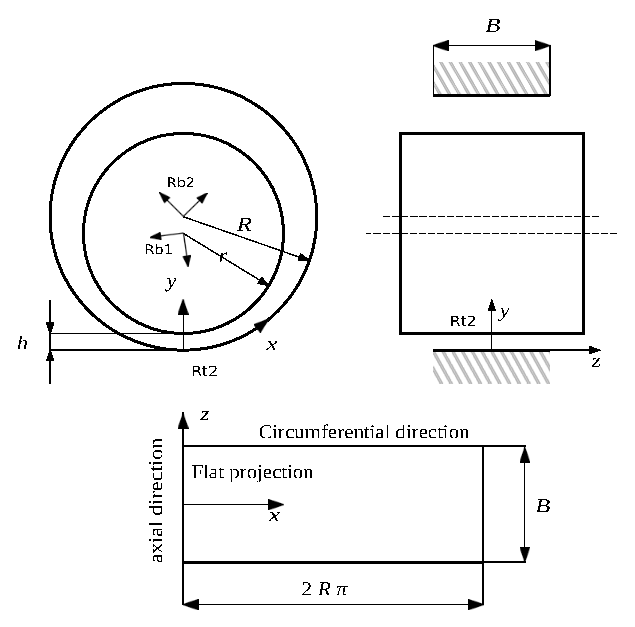
\includegraphics[width=0.5\linewidth]{fig_h100en}
\caption{Coordinate systems for cylindrical plain bearings}
\label{fig:h100}
\end{figure}

The $z$~axes of $\boldsymbol{R}_{b1}$ and $\boldsymbol{R}_{b2}$ correspond to the axes of the bearing journal and bearing shell. The $x$ and $y$~axis can be defined as required. The $x$~axis of $\boldsymbol{R}_{t2}$ is tangential to the circumference of the bearing shell, the $y$~axis is in the radial direction and the $z$~axis is parallel to the $z$~axis of $\boldsymbol{R}_{b2}$. The derivation of the Reynolds differential equation in section~\ref{sec:navier_stokes} is based on the coordinate system~$\boldsymbol{R}_{t2}$. However, $\boldsymbol{R}_{t1}$ could be used as well.

\subsection{Derivation of the Reynolds equation from the compressible Navier Stokes equation}
\label{sec:navier_stokes}
Since, according to \cite{Butenschoen-1976}, the radial gap height $h$ is small compared to the radius $R$, the curvature of the oil-filled gap can be neglected. For this reason, as shown in figure~\ref{fig:h100}, the volume of the gap can be unrolled onto a plane and the Navier Stokes equation can be written in Cartesian coordinates. If we assume a Newtonian fluid with constant viscosity and laminar flow, then according to \cite{DIRKBARTEL2010} the Navier Stokes equation given in equation~\ref{eq:h100} follows for the flow in $x$ and $z$~direction. As the flow velocity in the radial gap height direction is neglected, the Navier Stokes equation for the $y$~direction is not applicable.

\begin{IEEEeqnarray}{rCl}
\label{eq:h100}
\underbrace{\rho\,\left(\frac{\partial u_x}{\partial t} + u_x \, \frac{\partial u_x}{\partial x} + u_y \, \frac{\partial u_x}{\partial y} + u_z \, \frac{\partial u_x}{\partial z} \right)}_{\approx 0}&=&\underbrace{\rho\,g_x}_{\approx 0}-\frac{\partial p}{\partial x}+\underbrace{2\,\eta\,\frac{\partial^2 u_x}{\partial x^ 2}}_{\approx 0}-\frac{2}{3}\,\eta\,\left(\underbrace{\frac{\partial^2 u_x}{\partial x^2}}_{\approx 0}+\underbrace{\frac{\partial^2 u_y}{\partial x\,\partial y}}_{\approx 0} + \underbrace{\frac{\partial^2 u_z}{\partial x\,\partial z}}_{\approx 0}\right) \nonumber \\
&&+\eta\,\left(\frac{\partial^2 u_x}{\partial y^2} + \underbrace{\frac{\partial^2 u_y}{\partial x\,\partial y}}_{\approx 0}\right)+\eta\,\left(\underbrace{\frac{\partial^2 u_x}{\partial z^2}}_{\approx 0} + \underbrace{\frac{\partial^2 u_z}{\partial x\,\partial z}}_{\approx 0}\right) \nonumber \\
\underbrace{\rho\,\left(\frac{\partial u_z}{\partial t} + u_x \, \frac{\partial u_z}{\partial x} + u_y \, \frac{\partial u_z}{\partial y} + u_z \, \frac{\partial u_z}{\partial z}\right)}_{\approx 0}&=&\underbrace{\rho\,g_z}_{\approx 0}-\frac{\partial p}{\partial z}+\underbrace{2\,\eta\,\frac{\partial^2 u_z}{\partial z^2}}_{\approx 0}-\frac{2}{3}\,\eta\,\left(\underbrace{\frac{\partial^2 u_x}{\partial x\,\partial z}}_{\approx 0}+\underbrace{\frac{\partial^2 u_y}{\partial y\,\partial z}}_{\approx 0} + \underbrace{\frac{\partial^2 u_z}{\partial z^2}}_{\approx 0}\right) \nonumber \\
&&+\eta\,\left(\underbrace{\frac{\partial^2 u_x}{\partial x\,\partial z}}_{\approx 0} + \underbrace{\frac{\partial^2 u_z}{\partial x^2}}_{\approx 0}\right)+\eta\,\left(\underbrace{\frac{\partial^2 u_y}{\partial y\,\partial z}}_{\approx 0} + \frac{\partial^2 u_z}{\partial y^2}\right)
\end{IEEEeqnarray}

\begin{description}
\item[$\boldsymbol{u}=\begin{pmatrix} u_x \cr u_z \end{pmatrix}$] Flow velocity measured in the coordinate system $\boldsymbol{R}_{t1}$ or $\boldsymbol{R}_{t2}$\footnote{Strictly speaking, an inertial coordinate system would have to be used for the derivation. However, since the inertial forces are neglected in the derivation of Reynolds' differential equation, this does not matter}
\item[$p$] Fluid pressure
\item[$\rho$] Fluid density
\item[$\eta$] Dynamic viscosity of the fluid
\end{description}

According to \cite{Butenschoen-1976} and \cite{DIRKBARTEL2010}, the following simplifying assumptions can be made:
\begin{itemize}
\item Due to the small Reynolds numbers present in hydrodynamic plain bearings, the inertia forces can be neglected compared to the pressure forces and the frictional forces.
\item The gravity loads can also be neglected compared to the pressure forces and the frictional forces.
\item Since the radial gap height $h$ is very small compared to the bearing width $B$ and the bearing circumference $2\,R\,\pi$ for the usual bearing dimensions, the velocity gradients in $x$ and $z$~direction can be neglected in the friction terms compared to the velocity gradients in $y$ direction.
\item It is also assumed that the pressure change in the direction of the radial gap height is negligible. For the same reason, the Navier Stokes equation for the $y$ direction is also omitted.
\end{itemize}
With these assumptions, equation~\ref{eq:h100} is reduced to equation~\ref{eq:h200}.


\begin{IEEEeqnarray}{rCl}
\label{eq:h200}
\frac{\partial p}{\partial x} & = & \eta \, \frac{\partial^2 u_x}{\partial y^2} \nonumber \\
\frac{\partial p}{\partial z} & = & \eta \, \frac{\partial^2 u_z}{\partial y^2}
\end{IEEEeqnarray}

\subsubsection{Boundary conditions for the flow velocity at the bearing surface}
If it is assumed that the fluid adheres to the surface of the bearing journal and the surface of the bearing shell, the boundary conditions according to equation~\ref{eq:h300} apply\cite{Butenschoen-1976}. This requirement is usually fulfilled for radial plain bearings by selecting the appropriate bearing materials, as the adhesion condition is of decisive importance for the load carrying capacity of the bearing. For piston-cylinder bearings, however, adhesion to the surface is not absolutely necessary. For example, when using special coatings for pistons, the adhesion condition may not be fulfilled. This specific case, however, is excluded from this formulation.
\begin{IEEEeqnarray}{rCl}
\label{eq:h300}
\left. u_x \right\vert_{y=0}&=& \Delta U_{2x} \nonumber \\
\left. u_x \right\vert_{y=h}&=& \Delta U_{1x} \nonumber \\
\left. u_z \right\vert_{y=0}&=& \Delta U_{2z} \nonumber \\
\left. u_z \right\vert_{y=h}&=& \Delta U_{1z}
\end{IEEEeqnarray}

When introducing the boundary conditions, care must be taken to ensure that they are objective. A distinction is made between two cases:
\subparagraph{control volume moves with the bearing journal}
\begin{IEEEeqnarray}{rCl}
\Delta\boldsymbol{U}_1&=&\boldsymbol{0} \\
\Delta\boldsymbol{U}_2&=&\boldsymbol{U}_2 - \boldsymbol{U}_1
\end{IEEEeqnarray}

\subparagraph{control volume moves with the bearing shell}
\begin{IEEEeqnarray}{rCl}
\Delta\boldsymbol{U}_1&=&\boldsymbol{U}_1 - \boldsymbol{U}_2 \\
\Delta\boldsymbol{U}_2&=&\boldsymbol{0}
\end{IEEEeqnarray}

Obviously, the boundary conditions depend on the choice of control volume. However, the derivation of the radial gap height $\frac{\partial h}{\partial t}$ also depends on the choice of control volume. The kinematic relationships are discussed in section~\ref{sec:h100}.

\begin{description}
\item[$\boldsymbol{U}_1$] Absolute velocity at the surface of the bearing journal projected into the coordinate system $\boldsymbol{R}_{t1}$ or $\boldsymbol{R}_{t2}$
\item[$\boldsymbol{U}_2$] Absolute velocity at the surface of the bearing shell projected into the coordinate system $\boldsymbol{R}_{t1}$ or $\boldsymbol{R}_{t2}$
\item[$\Delta\boldsymbol{U}_1=\begin{pmatrix} \Delta U_{1x} \cr \Delta U_{1y} \cr \Delta U_{1z} \end{pmatrix}$] Velocity of the surface of the bearing journal relative to the control volume
\item[$\Delta\boldsymbol{U}_2=\begin{pmatrix} \Delta U_{2x} \cr \Delta U_{2y} \cr \Delta U_{2z} \end{pmatrix}$] Velocity of the surface of the bearing shell relative to the control volume
\end{description}

If equation~\ref{eq:h200} is integrated twice over the radial gap height and the boundary conditions \ref{eq:h300} are used, this results in a parabolic velocity distribution in the direction of the radial gap height\cite{Butenschoen-1976}, \cite{DIRKBARTEL2010}.
\begin{IEEEeqnarray}{rCl}
u_x&=&\frac{1}{\eta}\,\frac{\partial p}{\partial x}\,\left(\frac{y^2}{2} - y\,\frac{h}{2}\right) + \frac{\Delta U_{1x} - \Delta U_{2x}}{h}\,y + \Delta U_{2x} \nonumber \\
u_z&=&\frac{1}{\eta}\,\frac{\partial p}{\partial z}\,\left(\frac{y^2}{2} - y\,\frac{h}{2}\right) + \frac{\Delta U_{1z} - \Delta U_{2z}}{h}\,y + \Delta U_{2z}
\label{eq:h325}
\end{IEEEeqnarray}

For the mass flow per unit length through the boundary of the control volume, the following applies\cite{Butenschoen-1976}, \cite{DIRKBARTEL2010}
\begin{IEEEeqnarray}{rClrCl}
\dot{m}_x & = & \int_{y=0}^{y=h} \rho\,u_x\,dy & = & \rho \, \underbrace{\int_{y=0}^{y=h} u_x \,
dy}_{q_x}
\\
\dot{m}_z & = & \int_{y=0}^{y=h} \rho\,u_z\,dy & = & \rho \, \underbrace{\int_{y=0}^{y=h}
\,u_z\,dy}_{q_z}
\end{IEEEeqnarray}

It is assumed that the density $\rho$ is only a function of the pressure $p$. Since the pressure is assumed to be constant in the direction of the radial gap height, the density is also constant in the $y$~direction.

\begin{IEEEeqnarray}{rCl}
\dot{m}_x&=&\rho \, q_x \\
\dot{m}_z&=&\rho \, q_z \\
q_x &=& \underbrace{\frac{\Delta U_{1x} + \Delta U_{2x}}{2}\,h}_{\text{Couette term}}
                \underbrace{- \frac{h^3}{12\,\eta}\,\frac{\partial p}{\partial x}}_{\text{Poiseuille term}} \\
q_z & = & \underbrace{\frac{\Delta U_{1z} + \Delta U_{2z}}{2}\,h}_{\text{Couette term}}
                  \underbrace{- \frac{h^3}{12\,\eta}\,\frac{\partial p}{\partial z}}_{\text{Poiseuille term}}
\end{IEEEeqnarray}

The compressible Reynolds differential equation~\ref{eq:h350} follows from the application of the continuity equation to the infinitesimal volume element\cite{Butenschoen-1976}, \cite{DIRKBARTEL2010}. To close this equation, a relationship between pressure and density must be specified. This is the purpose of the cavitation model, which will be introduced in section~\ref{sec:h400}.
\begin{IEEEeqnarray}{rCl}
\label{eq:h350}
\underbrace{\frac{\partial}{\partial t}\left(\rho \, h\right)}_{a} & = & -\frac{\partial \dot{m}_x}{\partial x} -\frac{\partial \dot{m}_z}{\partial z} \nonumber \\
&=&-\frac{\partial}{\partial x} \, \left[\rho \, \left(\frac{\Delta U_{1x} + \Delta U_{2x}}{2} \, h - \frac{h^3}{12 \, \eta} \, \frac{\partial p}{\partial x} \right) \right] \nonumber \\
&&-\frac{\partial}{\partial z} \, \left[ \rho \, \left(\frac{\Delta U_{1z} + \Delta U_{2z}}{2} \, h - \frac{h^3}{12 \, \eta} \, \frac{\partial p}{\partial z} \right) \right]
\end{IEEEeqnarray}

\subsubsection{Micro hydrodynamic effects}
Equation~\ref{eq:h350} is valid for smooth and rough surfaces, as long as the resolution of the mesh is sufficiently high in order to capture the surface roughness profile at micrometer scale. Otherwise, the averaged Reynolds equation~\ref{eq:h351} according to Patir and Cheng must be used\cite{PatirCheng1978}. In equation~\ref{eq:h351} $\bar{h}_T$ is the average radial clearance considering the roughness profile, $\phi_x$ and $\phi_z$ are the pressure flow factors in $x$ and $z$-direction respectively, $\phi_{s_x}$ and $\phi_{s_z}$ are the shear flow factors in $x$ and $z$-direction respectively, and $\sigma_c=\sqrt{\sigma_1^2+\sigma_2^2}$ is the combined standard deviation of the roughness profiles of the bearing journal and shell surface. $\sigma_1$ and $\sigma_2$ are the standard deviations of the roughness profiles of the bearing journal and shell surface respectively.
\begin{IEEEeqnarray}{rCl}
\label{eq:h351}
\frac{\partial}{\partial t}\left(\rho \, \bar{h}_T\right) &=&-\frac{\partial}{\partial x} \, \left[\rho \, \left(\frac{\Delta U_{1x} + \Delta U_{2x}}{2} \, \bar{h}_T + \frac{\Delta U_{1x} - \Delta U_{2x}}{2} \, \sigma_c \, \phi_{s_x} - \phi_x \, \frac{h^3}{12 \, \eta} \, \frac{\partial p}{\partial x} \right) \right] \nonumber \\
&&-\frac{\partial}{\partial z} \, \left[\rho \, \left(\frac{\Delta U_{1z} + \Delta U_{2z}}{2} \, \bar{h}_T + \frac{\Delta U_{1z} - \Delta U_{2z}}{2} \, \sigma_c \, \phi_{s_z} - \phi_z \, \frac{h^3}{12 \, \eta} \, \frac{\partial p}{\partial z} \right) \right] \\
\bar{h}_T&=&\frac{h}{2}\left[1+erf\left(\frac{h}{\sqrt{2}\,\sigma_c}\right)\right]+\frac{\sigma_c}{\sqrt{2\pi}}\exp{\left(-\frac{h^2}{2\sigma_c^2}\right)}
\end{IEEEeqnarray}
\paragraph{Pressure flow factors}
The pressure flow factors are defined as\cite{PatirCheng1978}:
\begin{IEEEeqnarray}{rCl}
H&=&\frac{h}{\sigma_c} \\
\phi_x&=&\left\{\begin{array}{rcl} 1 - C\,\exp{\left(-r\,H\right)} & \text{if} & \gamma_c \leq 1 \\
                            1 + C\,H^{-r} & \text{if} & \gamma_c > 1
         \end{array}\right. \\
\phi_z\left(H, \gamma_c\right)&=&\phi_x\left(H, \frac{1}{\gamma_c}\right)
\end{IEEEeqnarray}
Where $C$ and $r$ are functions of the combined Peklenik factor $\gamma_c$, which are interpolated from table~\ref{tb:h360}. The combined Peklenik factor $\gamma_c$ is defined as:
\begin{IEEEeqnarray}{rCl}
\gamma_c&=&\frac{\frac{V_{r1}}{\lambda_{z1}} + \frac{V_{r2}}{\lambda_{z2}}}{\frac{V_{r1}}{\lambda_{x1}}+\frac{V_{r2}}{\lambda_{x2}}} \\
V_{r1}&=&\left(\frac{\sigma_1}{\sigma_c}\right)^2 \\
V_{r2}&=&\left(\frac{\sigma_2}{\sigma_c}\right)^2
\end{IEEEeqnarray}
Where $\sigma_1$ and $\sigma_2$ are the standard deviations of the roughness profiles from the bearing journal and shell surface respectively. $\lambda_{x1}$ and $\lambda_{x2}$ are the autocorrelation lengths in $x$-direction of the roughness profiles of the bearing journal and shell surface respectively. $\lambda_{z1}$ and $\lambda_{z2}$ are the corresponding autocorrelation lengths in $z$-direction.
Standard deviations and autocorrelation lengths can be determined from a profilometer trace of the respective bearing surface.
\begin{table}
\centering
\caption{Coefficients for the calculation of the pressure flow factors $\phi_x$ and $\phi_z$\cite{PatirCheng1978}}
\begin{tabular}{c|c|c}
\hline
$\gamma_c$ & $C$ & $r$ \\
\hline
1/9 & 1.48 & 0.42 \\
1/6 & 1.38 & 0.42 \\
1/3 & 1.18 & 0.42 \\
1 & 0.9 & 0.56 \\
3 & 0.225 & 1.5 \\
6 & 0.520 & 1.5 \\
9 & 0.870 & 1.5
\end{tabular}
\label{tb:h360}
\end{table}
\paragraph{Shear flow factors}
The shear flow factors are defined as\cite{PatirCheng1978}:
\begin{IEEEeqnarray}{rCl}
\phi_{s_x} & = & V_{r1} \, \Phi_{s}\left(H, \gamma_1\right) - V_{r2} \, \Phi_{s}\left(H, \gamma_2\right) \\
\phi_{s_z} & = & V_{r1} \, \Phi_{s}\left(H, \frac{1}{\gamma_1}\right) - V_{r2} \, \Phi_{s}\left(H, \frac{1}{\gamma_2}\right) \\
\Phi_s & = & \left\{\begin{array}{rcl} A_1\,H^{\alpha_1}\,\exp{\left(-\alpha_2\,H+\alpha_3\,H^2\right)} & \text{if} & H \leq 5 \\
A_2\,\exp{\left(-0.25\,H\right)} & \text{if} & H > 5
\end{array}\right. \\
\gamma_1 & = & \frac{\lambda_{x1}}{\lambda_{z1}} \\
\gamma_2 & = & \frac{\lambda_{x2}}{\lambda_{z2}}
\end{IEEEeqnarray}
Where $\gamma_1$ and $\gamma_2$ are the Peklenik factors of the bearing journal and shell surface respectively. $A_1$, $A_2$, $\alpha_1$, $\alpha_2$ and $\alpha_3$ are functions of the Peklenik factor of the corresponding bearing surface. Those values must be interpolated from table~\ref{tb:h370}.

\begin{table}
\centering
\caption{Coefficients for the calculation of the shear flow factors $\Phi_s$\cite{PatirCheng1978}}
\begin{tabular}{c|c|c|c|c|c}
\hline
$\gamma_1/\gamma_2$ & $A_1$ & $\alpha_1$ & $\alpha_2$ & $\alpha_3$ & $A_2$ \\
\hline
1/9 & 2.046 & 1.12 & 0.78 & 0.03 & 1.856 \\
1/6 & 1.962 & 1.08 & 0.77 & 0.03 & 1.754 \\
1/3 & 1.858 & 1.01 & 0.76 & 0.03 & 1.561 \\
1   & 1.899 & 0.98 & 0.92 & 0.05 & 1.126 \\
3   & 1.560 & 0.85 & 1.13 & 0.08 & 0.556 \\
6   & 1.290 & 0.62 & 1.09 & 0.08 & 0.388 \\
9   & 1.011 & 0.54 & 1.07 & 0.08 & 0.295 \\
\end{tabular}
\label{tb:h370}
\end{table}

\section{Cavitation models}
\label{sec:h400}
\subsection{Non-mass conserving cavitation}
\subsubsection{The incompressible Reynolds differential equation}
For the incompressible case, the density $\rho$ is constant\footnote{In fact the fluid will be incompressible if the Dowson-Higginson relation is not used, which is the default.}. This results in a linear partial differential equation of elliptic type with the pressure $p$ as an unknown.
\begin{IEEEeqnarray}{rCl}
\frac{\partial q_x}{\partial x} + \frac{\partial q_z}{\partial z} + \frac{\partial h}{\partial t} & = &
\frac{\partial}{\partial x}\left(\frac{\Delta U_{1x} + \Delta
U_{2x}}{2}\,h-\frac{h^3}{12\,\eta}\,\frac{\partial p}{\partial x}\right) \nonumber \\
&&+\frac{\partial}{\partial z}\left(\frac{\Delta U_{1z} + \Delta U_{2z}}{2}\,h -
\frac{h^3}{12\,\eta}\,\frac{\partial p}{\partial z}\right) + \frac{\partial h}{\partial t} = 0
\end{IEEEeqnarray}
\subsubsection{The G\"umbel boundary condition}
After discretization using finite differences or finite elements, a linear system of equations results. Since no cavitation model was used, its solution can contain negative pressures\cite{Butenschoen-1976}. According to \cite{Butenschoen-1976}, the negative pressures are set to zero after the solution of the linear system of equations in accordance with the G\"umbel boundary condition. However, this violates the continuity equation at the boundary of the cavitation region. According to \cite{Butenschoen-1976}, this causes an error in the pressure distribution. That error is increasing with the pressure gradient. The analytical solution of the incompressible Reynolds differential equation for an infinitely wide bearing given in \cite{Butenschoen-1976} results in a deviation in the Sommerfeld number between G\"umbel boundary condition and Reynolds boundary condition of $18\%$ with a relative eccentricity of $\varepsilon=0.999$ for the case of pure rotary motion\cite{Butenschoen-1976}. See also Figure~\ref{fig:h300}. Due to its simple implementation, the G\"umbel boundary condition was used for the incompressible case. With this method, however, it is not possible to calculate the amount of oil supplied via a lubrication groove as soon as the G\"umbel boundary condition becomes active, as the global conservation of mass is not fulfilled. Instead, the required oil quantity must be calculated from the volume flow that exits via the bearings boundaries.

\begin{figure}[htb]
\centering
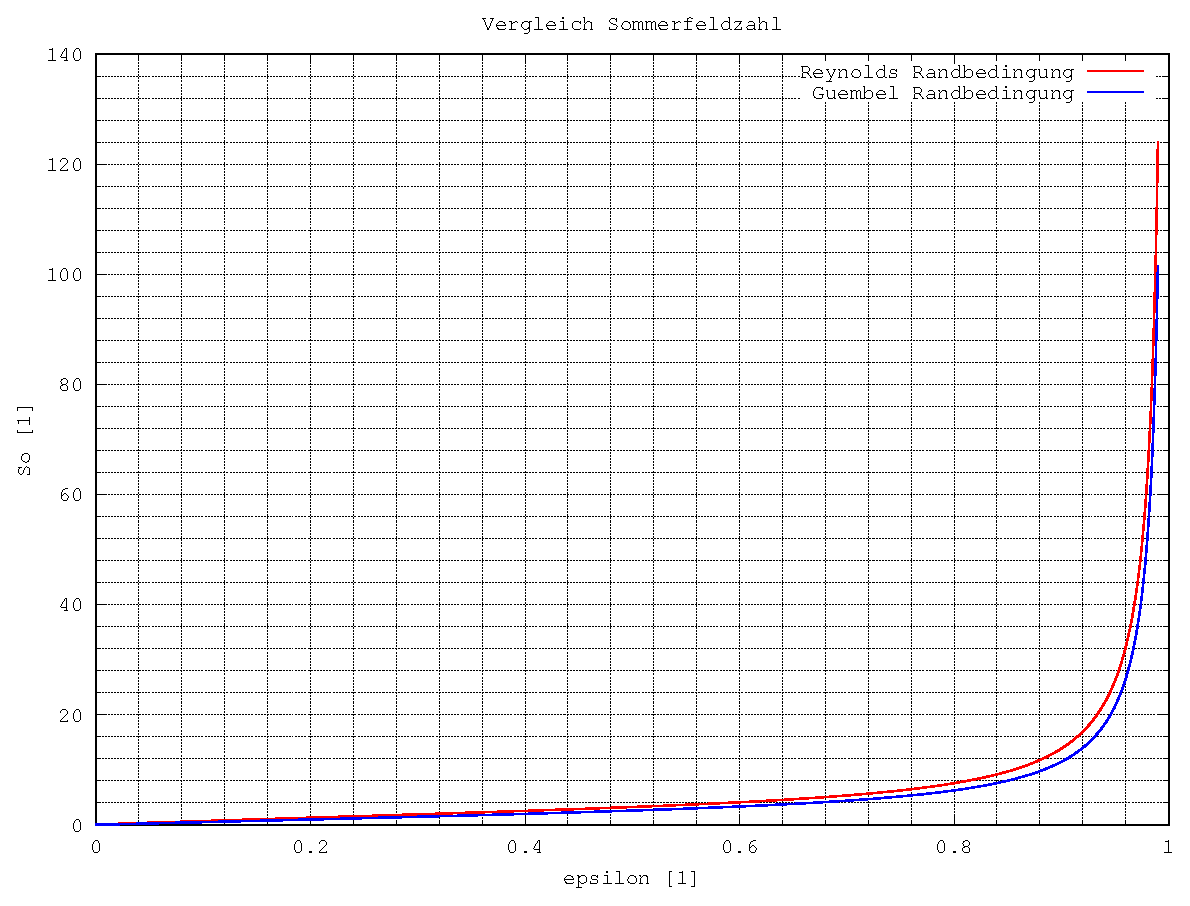
\includegraphics[width=0.5\linewidth]{fig_h300}
\caption[Differences between Reynolds boundary condition and G\"umbel boundary condition]{Differences in the Sommerfeld number between the Reynolds boundary condition and the G\"umbel boundary condition for the infinitely wide bearing with pure rotary motion}
\label{fig:h300}
\end{figure}

\subsubsection{The Reynolds boundary condition}
According to \cite{Butenschoen-1976}, the Reynolds boundary condition also requires that the pressure gradient is zero where the pressure is also zero. As a result, the continuity equation according to \cite{Butenschoen-1976} is fulfilled at least at the boundary of the cavitation region. In the cavitation region itself, however, the continuity equation is still not fulfilled according to \cite{DIRKBARTEL2010}. The implementation of the Reynolds boundary condition is much more difficult than the implementation of the G\"umbel boundary condition. In \cite{Butenschoen-1976}, for example, the pressures in the widest gap were iteratively adjusted to fulfill the Reynolds boundary condition. However, this method is only applicable in the case of a pure rotary motion. According to \cite{Bayada-2013}, it is possible to obtain the Reynolds boundary condition for the general case by setting the negative pressures to zero during the iterative solution of the linear system of equations using the Gauss Seidel method. However, this method only works if the matrices of the linear system of equations are symmetrically positive definite. As this is not the case in the multi-body system used, this method could not be implemented there. For test purposes, however, this method was implemented in a stand-alone finite element program for the solution of the incompressible Reynolds equation.

\subsection{Mass conserving cavitation}
\subsubsection{The Jakobsson Floberg Ollson (JFO) cavitation model}
According to \cite{Elrod-1981}, the so-called JFO cavitation model assumes that the flow in the cavitation region is divided into oil-filled strips and strips with oil vapor or dissolved gas. It is assumed that in the oil-filled strips the radial gap height is completely filled with oil. In the cavitation region where the mean density is less than the density of the liquid oil, the vapor pressure $p_c$ is uniform. This means that only Couette flow is possible in this region. In the full-film region where the pressure is greater than $p_c$, the fluid is assumed to be incompressible. The implementation of the JFO model is relatively complex as the boundaries of the cavitation region must be treated explicitly.
\subsubsection{The cavitation model of H. G. Elrod}
In \cite{Elrod-1981}, Elrod assumes in contrast to the JFO theory that the fluid in the full-film region is linearly compressible. The pressure is represented as a function of density.
\begin{IEEEeqnarray}{rCl}
p&=&p_c + g \, \beta \, \left(\Theta - 1\right) \nonumber \\
g & = & \left\{
\begin{array}{rcl}
1 & \text{if} & \Theta \geq 1 \\
0 & \text{if} & \Theta < 1
\end{array}
\right. \\
\Theta & = & \frac{\rho}{\rho_c}
\label{eq:h400}
\end{IEEEeqnarray}

\begin{description}
\item[$p_c$] Cavitation pressure
\item[$\rho_c$] Cavitation density
\item[$\beta$] bulk modulus
\item[$\Theta$] dimensionless density/pressure
\end{description}

By assuming a slightly compressible fluid, it is possible to calculate the distribution of pressure and density in the bearing without having to know the boundaries of the cavitation region. The problem is that the bulk modulus $\beta$ is very high, which affects the numerical stability. According to \cite{Luis-San-Andres-2010}, for example, the bulk modulus of mineral oil is $\beta=2.41GPa$. To avoid numerical stability problems, \cite{Luis-San-Andres-2010} often uses values for $\beta$ that are ten to one hundred times smaller than the physically correct bulk modulus. This circumstance was taken into account in \cite{Elrod-1981} by assuming the fluid to be incompressible for the calculation of the mass flows. The linear compressibility of the fluid is only taken into account in the term $a$ in equation~\ref{eq:h350}. According to \cite{Francisco-2009}, this makes it possible to artificially reduce the bulk modulus $\beta$ without affecting the results for the steady state. According to \cite{Francisco-2009}, the choice of the bulk modulus only affects the rate of convergence towards the steady state. However, an artificial reduction of $\beta$ is not applicable to transient analysis, because the orbital path would be undoubtedly affected.

\paragraph{The solution of the cavitation condition based on a mixed-complementarity problem}
Since the original Elrod model is not really applicable, it is necessary to modify the solution procedure. Instead of having only one unknown variable (e.g. either pressure $p$ or density $\rho$), it is necessary to solve for $p$ and $\rho$ simultaneously, and to add another inequality in order to make the mathematical problem well posed. This is a mixed nonlinear complementarity problem (MCP).
Now the complementarity condition describing the cavitation model is:
\begin{itemize}
\item If $p \geq 0$ then $\rho = \rho_{liquid}$
\item If $\rho$ < $\rho_{liquid}$ then $p = 0$
\end{itemize}
Where $\rho_{liquid}$ is the density of pure liquid without void fraction which is determined by equation~\ref{eq:h350b}. Actually $\rho >= 0$ is not a complementary condition but usually it is not hard to fulfill. In any case, it is necessary to use a dedicated nonlinear solver like \href{https://github.com/siconos/siconos}{SICONOS}, for the solution of this MCP. See also MBDyn's input manual about the nonlinear solvers which are usable for MCP's.

\subsubsection{Fluid properties}
So far, no assumptions have been made regarding the fluid viscosity $\eta$ and fluid density $\rho_{liquid}$. Actually MBDyn uses the Barus equation~\ref{eq:h350a} for the viscosity\cite{DIRKBARTEL2010} and the Dowson-Higginson equation~\ref{eq:h350b} for the density\cite{DIRKBARTEL2010}.
\begin{IEEEeqnarray}{rCl}
  \eta_{liquid} & = & \eta_c \, \exp{\left[\alpha_p\,\left(p - p_{c}\right)\right]} \label{eq:h350a}\\
  \rho_{liquid} & = & \rho_c \, \left[1 + \frac{ A_{\rho_1} \, \left(p - p_{c}\right)}{1 + A_{\rho_2} \, \left(p - p_{c}\right)}\right] \label{eq:h350b} \\
  \eta&=&\eta_{liquid}\,\frac{\rho}{\rho_{liquid}}
\end{IEEEeqnarray}
Where $\eta_{liquid}$ is the dynamic viscosity of the pure liquid without any void fraction, $\alpha_p$ is the pressure-viscosity coefficient and $\eta_c$ is the reference viscosity at pressure $p_c$. $\rho_c$ is the reference density at pressure $p_c$ and the coefficients for mineral oil are $A_{\rho_1}=0.6GPa^{-1}$ and $A_{\rho_2}=1.7GPa^{-1}$\cite{DIRKBARTEL2010}.

\section{Discretization of the Reynolds differential equation using finite differences}
\label{sec:h150}
\subsection{The orthogonal finite difference mesh of a cylindrical journal bearing}
Figure~\ref{fig:h150} shows the basic structure of such a mesh. The grid spacing does not have to be equidistant. For example, it is possible to refine the mesh in the areas of the piston skirt and the sealing edge of the piston. To make it easier to implement the periodic boundary condition of the cylindrical journal bearing with the five node elements, the mesh on the left-hand side was extended by one node beyond the physical boundary of the bearing surface. For each active node, a five-node element with that node in the center must be defined. The edge nodes of a five-node element can be active or passive nodes. The four node elements for reaction forces and axial mass flow are only located within the physical bearing surface.

\begin{figure}[htb]
\centering
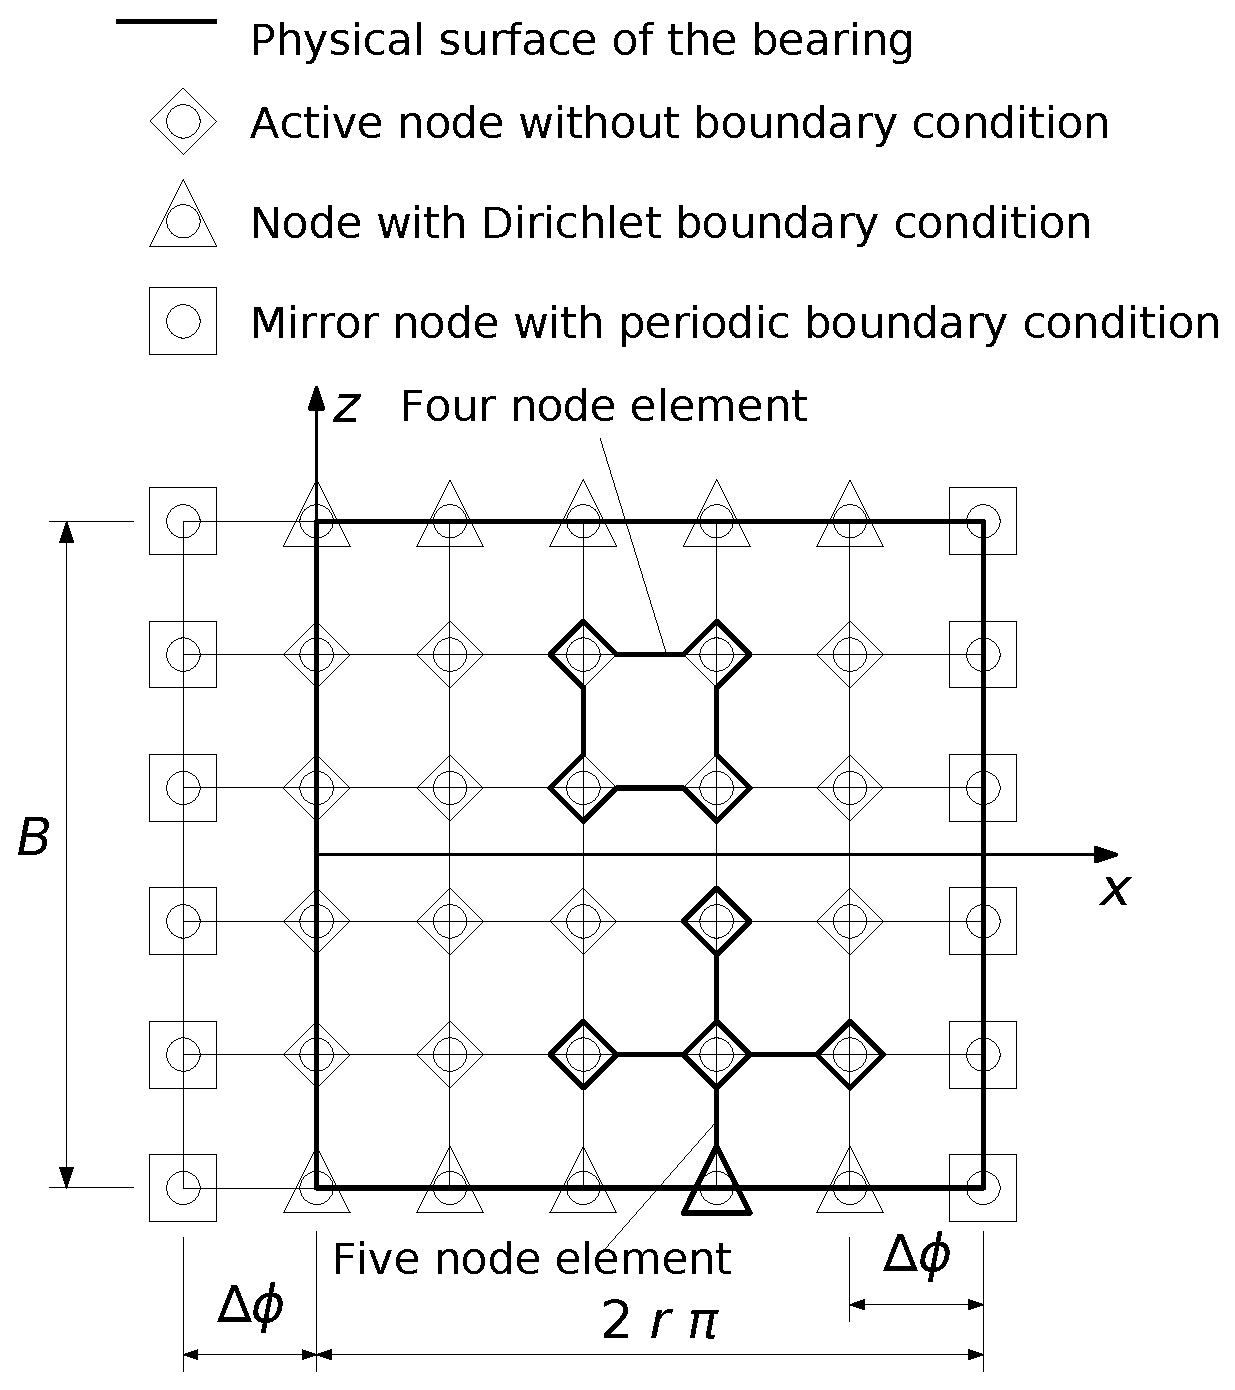
\includegraphics[width=0.5\linewidth]{fig_h150en}
\caption{orthogonal finite difference mesh of a cylindrical journal bearing}
\label{fig:h150}
\end{figure}

\subsection{The compressible Reynolds differential equation}
\begin{IEEEeqnarray}{rCl}
\left.\frac{\partial p}{\partial x} \right\vert_{\textit{wc}} & \approx & \frac{\left. p \right\vert_{\textit{center}} - \left. p \right\vert_{\textit{west}}}{\left. x \right\vert_{\textit{center}} -\left. x \right\vert_{\textit{west}}} \\
\left. h \right\vert_{\textit{wc}}&\approx&\frac{1}{2}\,\left(\left. h\right\vert_{\textit{west}} + \left. h \right\vert_{\textit{center}}\right) \\
\left. \phi_{s_x}\right\vert_{\textit{wc}}&\approx&\phi_{s_x}\left(\left. h \right\vert_{\textit{wc}}\right) \\
\left. \Delta U_{1x} \right\vert_{\textit{wc}} &\approx& \frac{1}{2}\,\left(\left. \Delta U_{1x} \right\vert_{\textit{west}} + \left. \Delta U_{1x} \right\vert_{\textit{center}}\right)\\
\left. \Delta U_{2x} \right\vert_{\textit{wc}} &\approx& \frac{1}{2}\,\left(\left. \Delta U_{2x} \right\vert_{\textit{west}} + \left. \Delta U_{2x} \right\vert_{\textit{center}}\right)\\
\left. q_x \right\vert_{\textit{wc}} & \approx & \frac{\left. \Delta U_{1x} \right\vert_{\textit{wc}} + \left. \Delta U_{2x} \right\vert_{\textit{wc}}}{2} \, \left. \bar{h}_T \right\vert_{\textit{wc}} + \frac{\left. \Delta U_{1x} \right\vert_{\textit{wc}} - \left. \Delta U_{2x} \right\vert_{\textit{wc}}}{2} \, \sigma_c \, \left.\phi_{s_x}\right\vert_{\textit{wc}} \nonumber\\
&&-\phi_x \, \frac{\left. h^3 \right\vert_{\textit{wc}}}{12\,\left.\eta\right\vert_{\textit{wc}}} \, \left. \frac{\partial p}{\partial x}\right\vert_{\textit{wc}} \\
\left. \rho \right\vert_{\textit{wc}} & \approx & \left\{
\begin{array}{ll}
    \left.\rho\right\vert_{\textit{west}} & \text{if} \qquad q_x\vert_{\textit{wc}} \geq 0 \\
    \left.\rho\right\vert_{\textit{center}} & \text{if} \qquad q_x\vert_{\textit{wc}} < 0
\end{array} \right. \\
\left. \eta \right\vert_{\textit{wc}} & \approx & \frac{1}{2} \, \left(\left.\eta\right\vert_{\textit{west}} + \left. \eta \right\vert_{\textit{center}} \right) \\
\dot{m}_x\vert_{\textit{wc}} & \approx & \left. \rho \right\vert_{\textit{wc}} \, \left. q_x \right\vert_{\textit{wc}} \\
\left. \frac{\partial \dot{m}_x}{\partial x} \right\vert_{\textit{center}} & \approx & \frac{\dot{m}_x\vert_{\textit{ce}} - \dot{m}_x\vert_{\textit{wc}}}{x\vert_{\textit{ce}} - x\vert_{\textit{wc}}} \\
\left. \frac{\partial \dot{m}_z}{\partial z} \right\vert_{\textit{center}} & \approx & \frac{\dot{m}_z\vert_{\textit{cn}} - \dot{m}_z\vert_{\textit{sc}}}{z\vert_{\textit{cn}} - z\vert_{\textit{sc}}} \\
\left. \frac{\partial}{\partial t}\,\left(\rho \, h\right)\right\vert_{\textit{center}} & \approx & \frac{\partial}{\partial t}\,\left(\left. \rho \right\vert_{\textit{center}} \, \left. h \right\vert_{\textit{center}}\right)
\end{IEEEeqnarray}

\subsubsection{The Courant Friedrichs Lewy condition}
Since the compressible Reynolds equation is of parabolic type, it is necessary to consider the CFL condition. This is for the two-dimensional case:
\begin{IEEEeqnarray}{rCl}
\Delta t & \leq & \frac{C_{max}}{\frac{q_x}{h\,\Delta x} + \frac{q_z}{h\,\Delta z}}
\end{IEEEeqnarray}
The CFL condition is checked in the multibody system in each iteration after the calculation of the residual, and the time step size is reduced accordingly if necessary. For explicit methods, $C_{max}=1$ usually applies. However, since the solution method used is implicit, it is also possible that $C_{max} \geq 1$ is specified. However, values of $C_{max}$ that are too high can lead to divergence of the non-linear solver.

\section{Hydraulic boundary conditions}
\subsection{Dirichlet boundary condition}
Dirichlet boundary conditions can be specified either for the hydraulic pressure $p$ or for the density $\rho$ or for the radial gap height $h_0$ filled with oil.

\subsubsection{Partially flooded boundaries of the bearing}
In this case, it is assumed that the component surface on the opposite side of the mesh is wetted with an oil film with a layer thickness of $h_0$ at the boundaries of the bearings. See figure~\ref{fig:h350}.
\begin{figure}[htb]
\centering
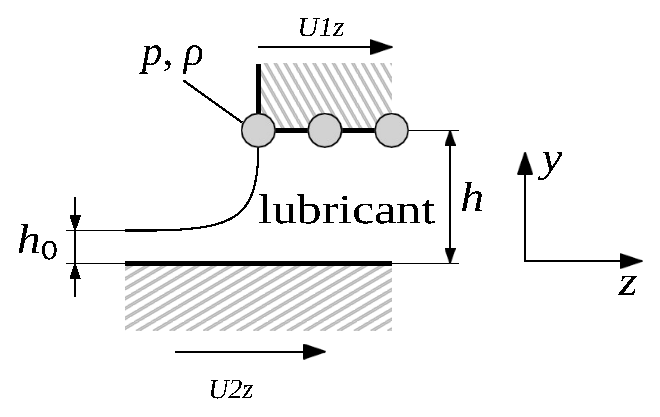
\includegraphics[width=0.5\linewidth]{fig_h350}
\caption{assumptions for partially flooded boundaries of the bearing}
\label{fig:h350}
\end{figure}
This assumption was made based on the commercial software AVL-Excite. In the case of the lubricating film of the piston, where the mesh is always on the piston side, an oil film with a layer of constant thickness $h_0$ on the cylinder liner is assumed, because only in this case it is possible to have oil transport through the boundaries of the bearing due to the axial movement of the piston. The fluid density at the boundaries of the bearing is determined as follows:
\begin{IEEEeqnarray}{rCl}
\Phi & = & \frac{h_0}{h} \\
\rho & = & \left\{
\begin{array}{ll}
\rho_c \, \Phi & \text{if} \qquad \Phi \leq 1 \cr
\rho_c & \text{if} \qquad \Phi > 1
\end{array}
\right.
\end{IEEEeqnarray}
However, since Reynolds' differential equation only knows one independent variable, it is not possible to specify density and pressure at the boundaries of the bearing at the same time. In order to be able to specify pressure and density independently of each other, it would be necessary to switch to a multiphase flow which also takes into account the proportion of dissolved gas. However, such an approach was not pursued.

\subsubsection{Coupling of boundary conditions with other variables}
When specifying a Dirichlet boundary condition, it is possible to specify not only constants but also any function as a boundary conditions. For example the pressure can be specified as a boundary condition for the lubricating film at the boundaries of a bearing, or within lubrication grooves, by means of a ``DriveCaller''. See also MBDyn's input manual.

\subsubsection{Geometric locations for the application of boundary conditions}
A Dirichlet boundary condition is always required at the boundaries of the bearing for cylindrical plain bearings. In addition, lubrication grooves with a circular or rectangular cross-section can be defined and Dirichlet boundary conditions can be specified there. For reasons of accuracy, the mesh must be located at the same side as the lubrication grooves.

\subsection{Periodic boundary conditions}
Since the surface of the cylindrical plain bearing is unwound onto a plane, it is necessary that the radial boundaries of the unwound bearing surface are coupled with each other. For this purpose, so-called mirror nodes were introduced which have their own nodal coordinates but obtain their value and equation number from their corresponding nodes at the opposite side of the mesh.

\subsection{Coupling of a plain bearing with a hydraulic network}
In MBDyn, it is also possible to set up hydraulic networks consisting of pipelines, valves, throttle points, tanks and hydraulic actuators. For this reason, it was obvious to provide a coupling between individual plain bearings with a hydraulic network. In this way, for example, two journal bearings may be connected to each other via a pipeline. The quantity of oil supplied via the oil pump can be specified as a function of the revolution speed, for example.

\subsubsection{Coupling at the boundaries of the bearing surface}
When coupling the mass flow through the boundaries of the bearing with the hydraulic network, the following conditions apply for the bearing boundary at $z=\frac{B}{2}$:
\begin{IEEEeqnarray}{rCl}
\left.p\right\vert_{z=\frac{B}{2}} & = & p_{hyd} \\
\dot{m}_{hyd} & = & -\int_{x=0}^{2\pi\,r} \left[\rho \, \left.\left(\frac{\Delta U_{1z} + \Delta
U_{2z}}{2} \, \bar{h}_T + \frac{\Delta U_{1z} - \Delta
U_{2z}}{2}\,\sigma_c\,\phi_{s_z} - \phi_{z}\,\frac{h^3}{12 \, \eta} \, \frac{\partial p}{\partial
z}\right)\right]\right\vert_{z=\frac{B}{2}} \, dx
\label{h:710}
\end{IEEEeqnarray}
\begin{description}
\item[$p_{hyd}$] Pressure of the node from the hydraulic network which is coupled to the axial boundary of the bearing
\item[$\dot{m}_{hyd}$] Mass flow which emerges from the hydraulic network
\end{description}

The negative sign in equation~\ref{h:710} results from the convention for defining the residual for the nodes in the hydraulic network. Equation~\ref{h:710} applies if the network is located on the bearing journal. Otherwise, it must be integrated over $\int_{x=0}^{2\,\pi\,R}$.
\paragraph{Consideration of the flow direction for $z=-\frac{B}{2}$}
Coupling with the hydraulic network is achieved using four node coupling elements at the axial boundaries of the bearing surface. To couple the mass flow in the negative $z$ direction, the nodal coordinates are swapped in the $x$ direction so that $dx$ becomes negative.

\subsubsection{Coupling with a radial lubrication groove}
When coupling with a radial lubrication groove, the continuity equation is extended by an additional source term.
\begin{IEEEeqnarray}{rCl}
\left. p \right\vert_{A_{hyd}} & = & p_{hyd} \\
\dot{m}_{hyd} & = & \int_{A_{hyd}} \left\{\frac{\partial \left(\rho \, \bar{h}_T\right)}{\partial t} +
\frac{\partial}{\partial x}\left[\rho \, \left(\frac{\Delta U_{1x} + \Delta U_{2x}}{2} \, \bar{h}_T + \frac{\Delta U_{1x} - \Delta U_{2x}}{2} \, \sigma_c \, \phi_{s_x} - \phi_x \, \frac{h^3}{12 \, \eta}
\, \frac{\partial p}{\partial x}\right)\right]\right. \nonumber \\
& & + \left.\frac{\partial}{\partial z}\left[\rho\,\left(\frac{\Delta U_{1z} + \Delta U_{2z}}{2}
\, \bar{h}_T + \frac{\Delta U_{1z} + \Delta U_{2z}}{2} \, \sigma_c \, \phi_{s_z} - \phi_z \, \frac{h^3}{12 \, \eta} \, \frac{\partial p}{\partial z}\right)\right]\right\} \, dA_{hyd}
\end{IEEEeqnarray}
\begin{description}
\item[$A_{hyd}$] Area of the radial lubrication groove on the bearing surface
\end{description}
Pressure losses due to flow restrictions when entering the lubricating oil bore must be explicitly modeled in the hydraulic network by means of a throttling point. Coupling with a radial lubrication groove is possible only if it is located on the side of the mesh.

\section{Kinematic boundary conditions}
\label{sec:h100}
The kinematic variables $h$, $\frac{\partial h}{\partial t}=\dot{h}$, $\Delta \boldsymbol{U}_1$ and $\Delta \boldsymbol{U}_2$ required in equation~\ref{eq:h350} are derived in this section. Two possibilities have been implemented so far:
\begin{itemize}
  \item The mesh moves with the bearing journal
  \item The mesh moves with the bearing shell
\end{itemize}
In the case of a piston-cylinder bearing, the first option must be selected so that the kinematic boundary conditions and the reaction forces correspond to reality. Both options can be used for radial plain bearings. The mesh must be located on the side where the lubrication grooves are located. However, it is also possible to specify pockets on the side opposite to the mesh.

\subsection{The cylindrical plain bearing in which the mesh moves with the bearing journal}
\label{sec:h200}
The kinematic relationships in Equation~\ref{eq:h_1000} are shown in Figure~\ref{fig:h400}. It is assumed that the radial gap height vector $\boldsymbol{v}_h$ is normal to the surface of the bearing shell. Other assumptions would lead to a quadratic equation with multiple solutions. However, with the bearing clearances of $\Psi \approx 10^{-3}$ that are usual for radial plain bearings, the approximation used should be more than sufficiently accurate. For piston-cylinder bearings, the relative bearing clearance is even smaller than that.

\begin{figure}[htb]
\centering
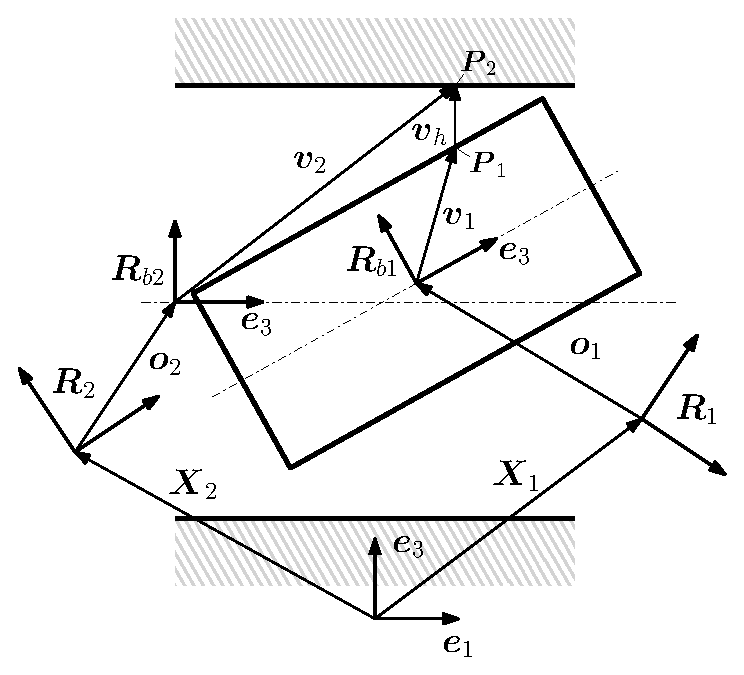
\includegraphics[width=0.5\linewidth]{fig_h400}
\caption{Kinematics of the rigid cylindrical plain bearing with mesh on the bearing journal}
\label{fig:h400}
\end{figure}

\subsubsection{The determination of the radial gap height}
\begin{IEEEeqnarray}{rCl}
\label{eq:h_1000}
\boldsymbol{X}_1 + \boldsymbol{R}_1 \, \left(\boldsymbol{o}_1 + \boldsymbol{R}_{b1} \,
\boldsymbol{v}_1\right) + \boldsymbol{R}_2 \, \boldsymbol{R}_{b2} \, \boldsymbol{v}_h & = &
\boldsymbol{X}_2 + \boldsymbol{R}_2 \, \left(\boldsymbol{o}_2 + \boldsymbol{R}_{b2} \,
\boldsymbol{v}_2\right)
\end{IEEEeqnarray}

\begin{description}
\item[$\boldsymbol{X}_1$] Position of the node of the bearing journal
\item[$\boldsymbol{R}_1$] Orientation of the node of the bearing journal
\item[$\boldsymbol{\omega}_1$] Angular velocity of the node of the bearing journal
\item[$\boldsymbol{o}_1$] Distance between the center of the bearing journal and the structural node of the bearing journal
\item[$\boldsymbol{R}_{b1}$] Orientation of the bearing journal relative to the node of the bearing journal
\item[$\boldsymbol{v}_1$] Distance from the center of the bearing journal to the point at the surface of the journal at which the radial gap height is measured, in the coordinate system of the journal
\item[$\boldsymbol{X}_2$] Position of the node of the bearing shell
\item[$\boldsymbol{R}_2$] Orientation of the node of the bearing shell
\item[$\boldsymbol{\omega}_2$] Angular velocity of the structural node of the bearing shell
\item[$\boldsymbol{o}_2$] Distance between the center of the bearing shell and the node of the bearing shell
\item[$\boldsymbol{R}_{b2}$] Orientation of the bearing shell relative to the structural node of the bearing shell
\item[$\boldsymbol{v}_2$] Distance from the center of the bearing shell to the point on the surface of the bearing shell at which the radial gap height is measured, in the coordinate system of the bearing shell
\item[$\boldsymbol{v}_h$] Vector of the radial gap height
\item[$h_{rb}$] Radial gap height, not considering elastic deformations of the bearing surfaces
\item[$h$] Actual radial gap height
\item[$w_{tot}$] Total radial component of the elastic deformation of the surfaces of bearing shell and bearing journal\footnote{The determination of ${w}_{tot}$ will be covered in section~\ref{sec:fsi_100}}.
\end{description}

For a certain node on the bearing journal, the vector $\boldsymbol{v}_1$ is known a priori according to equation~\ref{eq:h_1100}. The unknown variables in equation~\ref{eq:h_1200} and equation~\ref{eq:h_1300} are $\varphi_2$ and $h_{rb}$. These must be determined so that equation~\ref{eq:h_1000} is fulfilled.
\begin{IEEEeqnarray}{rCl}
\label{eq:h_1100}
\boldsymbol{v}_1 & = &
\begin{pmatrix}
\left(r + \Delta y_1\right) \, \cos\varphi_1 \cr
\left(r + \Delta y_1\right) \, \sin\varphi_1 \cr
z_1
\end{pmatrix} \\
\label{eq:h_1200}
\boldsymbol{v}_2 & = &
\begin{pmatrix}
\left(R + \Delta y_2\right) \, \cos\varphi_2 \cr
\left(R + \Delta y_2\right) \, \sin\varphi_2 \cr
z_2
\end{pmatrix} \\
\label{eq:h_1300}
\boldsymbol{v}_h & = &
\begin{pmatrix}
h_{rb} \, \cos\varphi_2 \\
h_{rb} \, \sin\varphi_2 \\
0
\end{pmatrix}
\end{IEEEeqnarray}
\begin{description}
\item[$\begin{pmatrix} \varphi_1 & z_1 \end{pmatrix}$] Position of the hydrodynamic node on the bearing journal in cylindrical coordinates
\item[$\Delta y_1$] Deviation of the journal surface with respect to the ideal cylindrical shape within specified areas (e.g. barrel shape, cone shape, ellipse shape, grooves, $\hdots$).
\item[$\begin{pmatrix} \varphi_2 & z_2 \end{pmatrix}$] Position of the point on the surface of the bearing shell which is opposite the hydrodynamic node on the bearing journal
\item[$\Delta y_2$] Deviation of the bearing shell surface with respect to the ideal cylindrical surface within specified areas (e.g. barrel shape, cone shape, ellipse shape, grooves, $\hdots$).
\end{description}

Due to the assumption that the vector $\boldsymbol{v}_h$ is normal to the surface of the bearing shell, the resolution of equation~\ref{eq:h_1000} to $\varphi_2$ and $h_{rb}$ is simple:
\begin{IEEEeqnarray}{rCl}
\boldsymbol{v}_2 -
\boldsymbol{v}_h & = & \underbrace{\boldsymbol{R}_{b2}^T \, \left\{\boldsymbol{R}_2^T \,
\left[\boldsymbol{X}_1 + \boldsymbol{R}_1 \, \left(\boldsymbol{o}_1 + \boldsymbol{R}_{b1} \, \boldsymbol{v}_1\right)
- \boldsymbol{X}_2\right]-\boldsymbol{o}_2\right\}}_{\boldsymbol{b}}
\end{IEEEeqnarray}
\begin{IEEEeqnarray}{rCl}
\begin{pmatrix}
\left[\left(R + \Delta y_2\right) - h_{rb}\right] \, \cos\varphi_2 \cr
\left[\left(R + \Delta y_2\right) - h_{rb}\right] \, \sin\varphi_2 \cr
z_2
\end{pmatrix} & = &
\begin{pmatrix}
b_1 \cr
b_2 \cr
b_3 \cr
\end{pmatrix} \\
\sin\varphi_2 & = & \frac{b_2}{\sqrt{b_1^2 + b_2^2}} \\
\cos\varphi_2 & = & \frac{b_1}{\sqrt{b_1^2 + b_2^2}} \\
\tan\varphi_2 & = & \frac{b_2}{b_1} \\
h_{rb} & = & R + \Delta y_2 - \sqrt{b_1^2 + b_2^2} \\
h & = & h_{rb} + w_{tot}
\end{IEEEeqnarray}

In addition, the derivatives of the radial gap height with respect to time are required for the Reynolds differential equation:
\begin{IEEEeqnarray}{rCl}
\dot{h}_{rb} & = & \Delta\dot{y}_2 - \frac{b_1 \, \dot{b}_1 + b_2 \, \dot{b}_2}{\sqrt{b_1^2 + b_2^2}}
\\
\dot{h} & = & \dot{h}_{rb} + \dot{w}_{tot} \\
\dot{\boldsymbol{b}} & = & \boldsymbol{R}_{b2}^T \, \boldsymbol{R}_2^T \,
\left\{\dot{\boldsymbol{X}}_1 + \left\langle \boldsymbol{\omega}_1 \right\rangle \,
\boldsymbol{R}_1 \, \left(\boldsymbol{o}_1 + \boldsymbol{R}_{b1} \, \boldsymbol{v}_1 \right)
- \dot{\boldsymbol{X}}_2 \right.\nonumber \\
& & \left.- \left\langle \boldsymbol{\omega}_2 \right\rangle \left[
\boldsymbol{X}_1 + \boldsymbol{R}_1 \, \left(\boldsymbol{o}_1 + \boldsymbol{R}_{b1} \,
\boldsymbol{v}_1 \right) - \boldsymbol{X}_2 \right]\right\}
\\
\Delta\dot{y}_2 & = & \frac{\partial \Delta y_2}{\partial x_2} \, \dot{x}_2 + \frac{\partial
\Delta y_2}{\partial z_2} \, \dot{z}_2 \\
\dot{x}_2 & = & R \, \dot{\varphi}_2 \\
\dot{\varphi}_2 & = & \frac{b_1 \, \dot{b}_2 - \dot{b}_1 \, b_2}{b_1^2 + b_2^2} \\
\dot{z}_2 & = & \dot{b}_3
\end{IEEEeqnarray}

For this purpose, the derivatives of $\Delta y_2$ must be specified.

\subsubsection{Deviations from the cylindrical bearing geometry}
Various types of so-called pockets were implemented. A pocket is a deviation from the cylindrical bearing geometry within a given boundary. Rectangular and circular boundaries are currently implemented. If a node is located within this boundary, then $\Delta y_1$ or $\Delta y_2$ correspond to the height of the respective pocket. In the case of a circular boundary, this is of course only a very rough approximation. In the case of a rectangular boundary, it is still possible to align the grid lines accordingly when generating the mesh.
\paragraph{Pocket with constant height $\Delta y$}
In this case, the specified height $\Delta y$ applies to the entire area within the boundary. This means that $\frac{\partial \Delta y}{\partial x}=0$ and $\frac{\partial \Delta
y}{\partial z}=0$.

\paragraph{Pocket with linear interpolation of $\Delta y$}
With linear interpolation, the height $\Delta y$ can be specified at four vertices of a rectangle. See figure~\ref{fig:h500}. The rectangle is only used for interpolation or extrapolation. The boundary of the pocket, on the other hand, can also be a circle, for example.

\begin{figure}[htb]
\centering
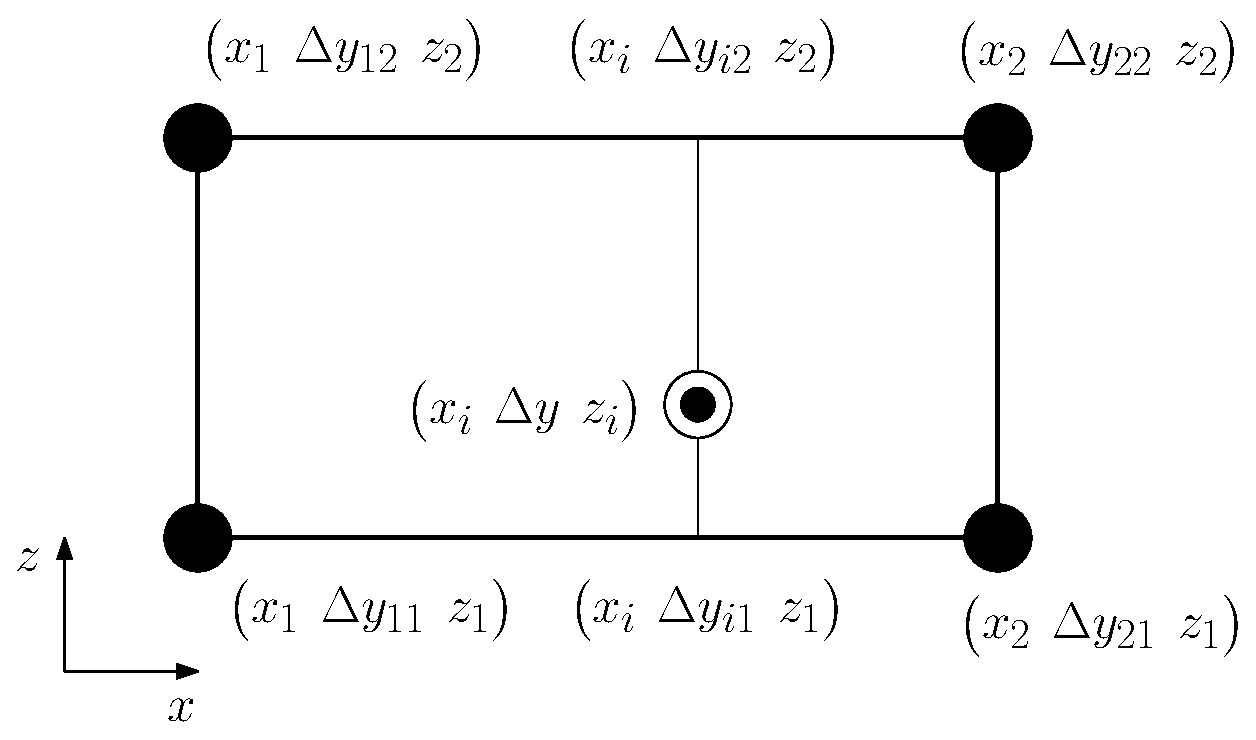
\includegraphics[width=0.5\linewidth]{fig_h500}
\caption{Interpolation of $\Delta y$ for a rectangular pocket}
\label{fig:h500}
\end{figure}

\begin{IEEEeqnarray}{rCl}
\Delta y_{i1} & = & \left(\Delta y_{21} - \Delta y_{11}\right) \, \frac{x_i - x_1}{x_2 - x_1} +
\Delta y_{11} \\
\Delta y_{i2} & = & \left(\Delta y_{22} - \Delta y_{12}\right) \, \frac{x_i - x_1}{x_2 - x_1} +
\Delta y_{12} \\
\Delta y & = & \left(\Delta y_{i2} - \Delta y_{i1}\right) \, \frac{z_i - z_1}{z_2 - z_1} +
\Delta y_{i1} \\
\frac{\partial \Delta y}{\partial x} & = & \frac{z_i - z_1}{z_2 - z_1} \,
\left(\frac{\partial \Delta y_{i2}}{\partial x} - \frac{\partial \Delta y_{i1}}{\partial x}\right) +
\frac{\partial \Delta y_{i1}}{\partial x} \\
\frac{\partial \Delta y_{i1}}{\partial x} & = & \frac{\Delta y_{21} - \Delta y_{11}}{x_2 - x_1} \\
\frac{\partial \Delta y_{i2}}{\partial x} & = & \frac{\Delta y_{22} - \Delta y_{12}}{x_2 - x_1} \\
\frac{\partial \Delta y}{\partial z} & = & \frac{\Delta y_{i2} - \Delta y_{i1}}{z_2 - z_1}
\end{IEEEeqnarray}

\subsubsection{boundary conditions for the velocities}
The velocities $\Delta\boldsymbol{U}_1$ and $\Delta\boldsymbol{U}_2$ must still be specified for the Reynolds differential equation. For this purpose, the velocity of the points $\boldsymbol{P}_1$ and $\boldsymbol{P}_2$ which are located on the surface of the bearing journal and bearing shell are first determined as shown in figure~\ref{fig:h400}.
\begin{IEEEeqnarray}{rCl}
\boldsymbol{P}_1 & = & \boldsymbol{X}_1 + \boldsymbol{R}_1 \, \left(\boldsymbol{o}_1 +
\boldsymbol{R}_{b1} \, \boldsymbol{v}_1\right) \\
\boldsymbol{P}_2 & = & \boldsymbol{X}_2 + \boldsymbol{R}_2 \, \left(\boldsymbol{o}_2 +
\boldsymbol{R}_{b2} \, \boldsymbol{v}_2 \right)
\end{IEEEeqnarray}

For the absolute velocities of the points $\boldsymbol{P}_1$ and $\boldsymbol{P}_2$ we get
\begin{IEEEeqnarray}{rCl}
\dot{\boldsymbol{P}}_1 & = & \dot{\boldsymbol{X}}_1 +
\left\langle \boldsymbol{\omega}_1 \right\rangle \, \boldsymbol{R}_1 \,
\left(\boldsymbol{o}_1 + \boldsymbol{R}_{b1} \, \boldsymbol{v}_1 \right) \\
\dot{\boldsymbol{P}}_2 & = & \dot{\boldsymbol{X}}_2 + \left\langle \boldsymbol{\omega}_2
\right\rangle \, \boldsymbol{R}_2 \, \left(\boldsymbol{o}_2 + \boldsymbol{R}_{b2} \,
\boldsymbol{v}_2 \right) - \left\langle\boldsymbol{\omega}_1\right\rangle\,\boldsymbol{R}_2\,\boldsymbol{R}_{b2}\,\boldsymbol{v}_h
\end{IEEEeqnarray}

Finally, the difference between the absolute velocities of the component surface and the control volume is transformed into the tangential coordinate system $\boldsymbol{R}_{t1}$. The orientation of the tangential coordinate system is shown in Figure~\ref{fig:h_700}. Since the mesh moves with the bearing journal according to the assumptions in this section, the velocity difference $\Delta\boldsymbol{U}_1$ at the bearing journal is zero.

\begin{IEEEeqnarray}{rCl}
\Delta\boldsymbol{U}_1 & = & \boldsymbol{0} \\
\Delta \boldsymbol{U}_2 & = & \boldsymbol{R}_{t1}^T \, \boldsymbol{R}_{b1}^T \, \boldsymbol{R}_1^T
\, \left(\dot{\boldsymbol{P}}_2 - \dot{\boldsymbol{P}}_1\right) \\
\boldsymbol{R}_{t1} & = & \begin{pmatrix}
-\sin\varphi_1 & -\cos\varphi_1 & 0 \cr
\cos\varphi_1 & -\sin\varphi_1 & 0 \cr
0 & 0 & 1
\end{pmatrix}
\end{IEEEeqnarray}

\begin{figure}[htb]
\centering
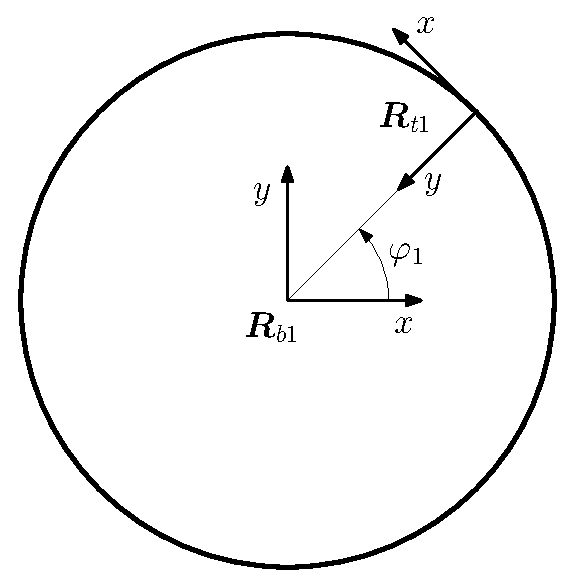
\includegraphics[width=0.3\linewidth]{fig_h700}
\caption{Orientation of the tangential coordinate system}
\label{fig:h_700}
\end{figure}

\subsection{The cylindrical plain bearing in which the mesh moves with the bearing shell}
It is assumed that the radial gap height $\boldsymbol{v}_h$ is measured normal to the surface of the bearing journal. See figure~\ref{fig:h600}. Apart from this, the kinematic relationships are the same as in section~\ref{sec:h200}.
\begin{figure}[htb]
\centering
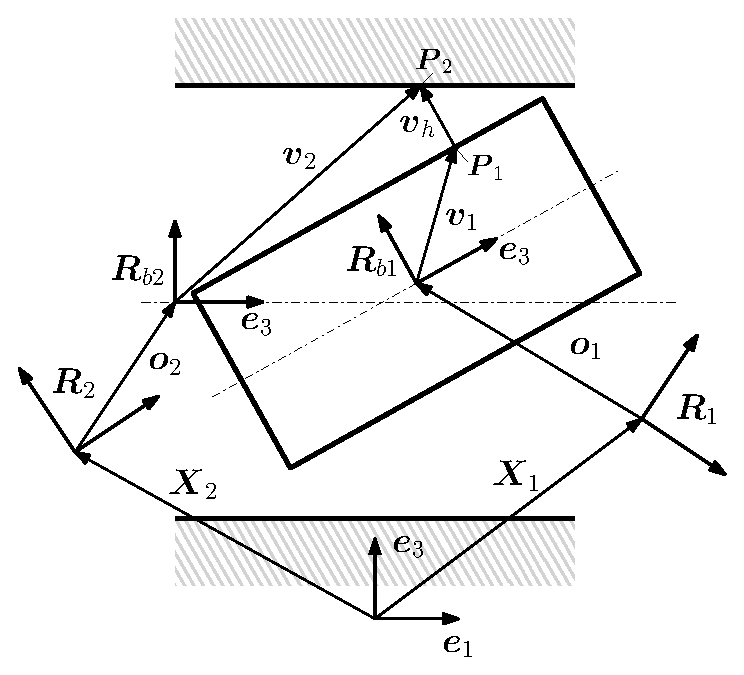
\includegraphics[width=0.5\linewidth]{fig_h600}
\caption{Kinematics of the cylindrical plain bearing with mesh on the bearing shell}
\label{fig:h600}
\end{figure}

\subsubsection{The determination of the radial gap height}
\begin{IEEEeqnarray}{rCl}
\boldsymbol{v}_h & = &
\begin{pmatrix}
h_{rb} \, \cos\varphi_1 \cr
h_{rb} \,  \sin\varphi_1 \cr
0 \end{pmatrix} \\
\boldsymbol{v}_1 + \boldsymbol{v}_{h} & = & \boldsymbol{b} \nonumber \\
& = & \boldsymbol{R}_{b1}^T
\, \left\{ \boldsymbol{R}_1^T \, \left[\boldsymbol{X}_2 + \boldsymbol{R}_2 \, \left(\boldsymbol{o}_2 + \boldsymbol{R}_{b2} \,
\boldsymbol{v}_2 \right) - \boldsymbol{X}_1\right] - \boldsymbol{o}_1 \right\} \\
\dot{\boldsymbol{b}} & = & \boldsymbol{R}_{b1}^T \, \boldsymbol{R}_1^T \, \left\{\dot{X}_2 +
\left\langle \boldsymbol{\omega}_2 \right\rangle \, \boldsymbol{R}_2 \,
\left(\boldsymbol{o}_2 + \boldsymbol{R}_{b2} \, \boldsymbol{v}_2\right) - \dot{\boldsymbol{X}}_1
\right. \nonumber \\
& & \left.- \left\langle\boldsymbol{\omega}_1\right\rangle \, \left[\boldsymbol{X}_2 +
\boldsymbol{R}_2 \, \left(\boldsymbol{o}_2 + \boldsymbol{R}_{b2} \, \boldsymbol{v}_2\right) -
\boldsymbol{X}_1\right]\right\} \\
\end{IEEEeqnarray}


\begin{IEEEeqnarray}{rCl}
\label{eq:h_1400}
\sin\varphi_1 & = & \frac{b_2}{\sqrt{b_1^2 + b_2^2}} \\
\cos\varphi_1 & = & \frac{b_1}{\sqrt{b_1^2 + b_2^2}} \\
\tan\varphi_1 & = & \frac{b_2}{b_1} \\
\dot{\varphi}_1 & = & \frac{b_1 \, \dot{b}_2 - \dot{b}_1 \, b_2}{b_1^2 + b_2^2} \\
h_{rb} & = & \sqrt{b_1^2 + b_2^2} - r - \Delta y_1 \\
\dot{h}_{rb} & = & \frac{b_1 \, \dot{b}_1 + b_2 \, \dot{b}_2}{\sqrt{b_1^2 + b_2^2}} - \Delta\dot{y}_1 \\
h & = & h_{rb} + w_{tot} \\
\dot{h} & = & \dot{h}_{rb} + \dot{w}_{tot} \\
\Delta\dot{y}_1 & = & \frac{\partial \Delta y_1}{\partial x_1} \, \dot{x}_1 + \frac{\partial\Delta y_1}{\partial z_1}\,\dot{z}_1 \\
\dot{x}_1 & = & r \, \dot{\varphi}_1 \\
\dot{z}_1 & = & \dot{b}_3
\end{IEEEeqnarray}

\subsubsection{Boundary conditions for the velocities}
In contrast to section~\ref{sec:h200}, the following applies to the velocities:
\begin{IEEEeqnarray}{rCl}
\dot{\boldsymbol{P}}_1 & = & \dot{\boldsymbol{X}}_1 +
\left\langle \boldsymbol{\omega}_1 \right\rangle \, \boldsymbol{R}_1 \,
\left(\boldsymbol{o}_1 + \boldsymbol{R}_{b1} \, \boldsymbol{v}_1 \right) + \left\langle\boldsymbol{\omega}_2\right\rangle\,\boldsymbol{R}_1\,\boldsymbol{R}_{b1}\,\boldsymbol{v}_h \\
\dot{\boldsymbol{P}}_2 & = & \dot{\boldsymbol{X}}_2 + \left\langle \boldsymbol{\omega}_2
\right\rangle \, \boldsymbol{R}_2 \, \left(\boldsymbol{o}_2 + \boldsymbol{R}_{b2} \,
\boldsymbol{v}_2 \right) \\
\Delta \boldsymbol{U}_1 & = & \boldsymbol{R}_{t2}^T \, \boldsymbol{R}_{b2}^T \, \boldsymbol{R}_2^T
\, \left(\dot{\boldsymbol{P}}_1 - \dot{\boldsymbol{P}}_2\right) \\
\Delta \boldsymbol{U}_2 & = & \boldsymbol{0}\\
\boldsymbol{R}_{t2} & = & \begin{pmatrix}
-\sin\varphi_2 & -\cos\varphi_2 & 0 \cr
\cos\varphi_2 & -\sin\varphi_2 & 0 \cr
0 & 0 & 1
\end{pmatrix}
\end{IEEEeqnarray}

\section{Solid body contact and dry friction}
\subsection{The contact model of Greenwood and Tripp}
In order to account for solid contact and dry friction between rough surfaces, the approach of Greenwood and Tripp was applied\cite{Greenwood-1970}. The equations for the Hertzian contact pressure between asperities of rough surfaces are \cite{Greenwood-1970}:
\begin{IEEEeqnarray}{rCl}
p_{asp} & = & \frac{16\,\sqrt{2}}{15} \, \pi \, \left(\eta_{asp} \, \beta_{asp} \sigma_{\delta}\right)^2
\, \acute{E} \, \sqrt{\frac{\sigma_{\delta}}{\beta_{asp}}} \,
F_{\frac{5}{2}}\left(\frac{h}{\sigma_{\delta}}\right) \\
\acute{E} & = & \left(\frac{1 - \nu_1^2}{E_1} + \frac{1 - \nu_2^2}{E_2}\right)^{-1} \\
F_{\frac{5}{2}}\left(H\right) & = & \left\{
\begin{array}{ll}
4.4086 \cdot 10^{-5} \, \left(4 -H\right)^{6.804} & \text{if} \qquad H \leq 4 \cr
0 & \text{if} \qquad H > 4
\end{array} \right. \\
H &=& \frac{h}{\sigma_{\delta}} \\
\sigma_{\delta} & = & \sqrt{M_0} \\
\eta_{asp} & = & \frac{1}{6 \, \pi \, \sqrt{3}} \, \frac{M_4}{M_2} \\
\beta_{asp} & = & \frac{3 \, \sqrt{\pi}}{8 \, \sqrt{M_4}}
\end{IEEEeqnarray}
\begin{description}
\item[$p_{asp}$] Pressure due to contact between the asperities of the rough surfaces
\item[$\eta_{asp}$] Asperity density
\item[$\beta_{asp}$] Radius of curvature of the asperity tip
\item[$\sigma_{\delta}$] Variance of the measured values of the roughness profile
\item[$M_0=\sigma_{\delta}^2$] combined zeroth spectral moment to describe the surface roughness
\item[$M_2=\dot{\sigma}_{\delta}^2$] combined second spectral moment to describe the surface roughness
\item[$M_4=\ddot{\sigma}_{\delta}^2$] combined fourth spectral moment to describe the surface roughness
\end{description}

According to \cite{Tomanik-2003}, those values can be determined from the analysis of measured roughness profiles of the component surfaces.

\subsection{The two-dimensional LuGre solid friction model} \label{sec:h500}
The standard model for the description of dry friction between solid bodies is Coulomb's law. However, the implementation of the transition between sliding friction and static friction for the general two-dimensional case is not trivial. The consideration of this transition is always important in a multi-body system, if the relative movement of a mechanism is going to stop due to friction. If sliding friction were always used in the calculation, an explicit integration scheme would result in endless oscillations around the static equilibrium point. For this reason, the two-dimensional LuGre model presented in \cite{LuGre2D} was selected, which is based on a linear differential equation and does not require any case distinctions. The LuGre friction model assumes that two bodies with rough surfaces touch each other at the tips of the asperities, also called bristles in the literature. With small relative movements, these bristles behave like springs. However, as soon as a certain maximum deformation is reached, the bristles begin to slide over each other. However, the transition between sticking and sliding is continuous in the LuGre model. The two-dimensional LuGre model from \cite{LuGre2D} reads:
\begin{IEEEeqnarray}{rCl}
\boldsymbol{\tau}_{asp} & = & \left(\boldsymbol{\sigma}_0 \, \boldsymbol{z} +
\boldsymbol{\sigma}_1
\,
\dot{\boldsymbol{z}}\right) \, p_{asp} \\
\dot{\boldsymbol{z}} & = & \Delta\boldsymbol{U} - \kappa \,
\boldsymbol{M}_{k}^{-2} \, \boldsymbol{\sigma}_0 \, \boldsymbol{z} \\
g & = & \frac{\left\Vert \boldsymbol{M}_k^2 \, \Delta\boldsymbol{U} \right\Vert}{\left\Vert
\boldsymbol{M}_k \, \Delta\boldsymbol{U}\right\Vert} + \left(\frac{\left\Vert \boldsymbol{M}_s^2 \, \Delta\boldsymbol{U} \right\Vert}{\left\Vert
\boldsymbol{M}_s \, \Delta\boldsymbol{U}\right\Vert} - \frac{\left\Vert \boldsymbol{M}_k^2 \, \Delta\boldsymbol{U} \right\Vert}{\left\Vert
\boldsymbol{M}_k \, \Delta\boldsymbol{U}\right\Vert}\right)\,\exp{\left[-\left(\frac{\left\Vert
\Delta\boldsymbol{U}\right\Vert}{v_s}\right)^\gamma\right]} \\
\kappa & = & \frac{\left\Vert \boldsymbol{M}_k^2 \, \Delta\boldsymbol{U}\right\Vert}{g} \\
\boldsymbol{M}_k & = & \begin{pmatrix}
\mu_{kx} & 0 \cr
0 & \mu_{kz}
\end{pmatrix} \\
\boldsymbol{M}_s & = & \begin{pmatrix}
\mu_{sx} & 0 \cr
0 & \mu_{sz}
\end{pmatrix} \\
\boldsymbol{\sigma}_0 & = & \begin{pmatrix}
\sigma_{0x} & 0 \cr
0 & \sigma_{0z}
\end{pmatrix} \\
\boldsymbol{\sigma}_1 & = & \begin{pmatrix}
\sigma_{1x} & 0 \cr
0 & \sigma_{1z}
\end{pmatrix} \\
\Delta\boldsymbol{U} & = & \begin{pmatrix}
\boldsymbol{e}_1^T \cr
\boldsymbol{e}_3^T
\end{pmatrix} \,
\left(\Delta\boldsymbol{U}_1 - \Delta\boldsymbol{U}_2\right)
\end{IEEEeqnarray}
\begin{description}
\item[$\boldsymbol{z} = \begin{pmatrix} z_1 \cr z_2 \end{pmatrix}$] Deformation of the bristles
\item[$\boldsymbol{\tau}_{asp} = \begin{pmatrix} \tau_{asp_{xy}} \cr
\tau_{asp_{yz}}\end{pmatrix}$] Shear stresses due to dry friction
\item[$\Delta\boldsymbol{U}$] Components of the velocity difference in $x$- and $z$~direction
\item[$\boldsymbol{\sigma}_0$] transient micro-sliding stiffness matrix
\item[$\boldsymbol{\sigma}_1$] transient micro-slip damping matrix
\item[$\boldsymbol{M}_k$] sliding friction matrix
\item[$\mu_{kx}$] coefficient of sliding friction in $x$~direction
\item[$\mu_{kz}$] Sliding friction coefficient in $z$~direction
\item[$\boldsymbol{M}_s$] static friction matrix
\item[$\mu_{sx}$] Coefficient of static friction in $x$~direction
\item[$\mu_{sz}$] Coefficient of static friction in $z$~direction
\item[$v_s$] Velocity which describes the transition between static friction and dynamic friction (Stribeck effect)
\item[$\gamma$] Coefficient that describes the transition between static friction and dynamic friction (Stribeck effect)
\end{description}

\subsubsection{The transition to Coulomb's law of friction}
For the stationary sliding process for isotropic surfaces without Stribeck effect, the LuGre model can be simplified as follows for illustrative purposes:
\begin{IEEEeqnarray}{rClrCl}
\dot{\boldsymbol{z}} & = & \boldsymbol{0}  \\
\boldsymbol{M}_k & = & \boldsymbol{M}_s \label{eq:h723} \\
\sigma_{0x} & = & \sigma_{0z} & = & \sigma_0 \label{eq:h724} \\
\mu_{kx} & = & \mu_{kz} & = & \mu_k \label{eq:h725}
\end{IEEEeqnarray}
With these simplifications we get
\begin{IEEEeqnarray}{rCl}
\boldsymbol{z} & = & \frac{\mu_k}{\sigma_0 \, \left\Vert \Delta\boldsymbol{U}\right\Vert_2} \,
\Delta\boldsymbol{U} \\
\boldsymbol{\tau}_{asp} & = & \boldsymbol{\sigma}_0 \, \boldsymbol{z} \, p_{asp} \nonumber \\
& = & \frac{\mu_k \, p_{asp}}{\left\Vert \Delta\boldsymbol{U} \right\Vert_2} \, \Delta\boldsymbol{U}
\label{eq:h750}
\end{IEEEeqnarray}
Equation~\ref{eq:h750} therefore corresponds exactly to the surface of the friction cone in Coulomb's law of friction.

\subsubsection{The transition to static friction}
For the unsteady one-dimensional case, the simplifications of equation~\ref{eq:h723}-\ref{eq:h725}:
\begin{IEEEeqnarray}{rCl}
\dot{z}_x & = & \Delta U_x - \left\vert \Delta U_x \right\vert \, \frac{\sigma_{0x}}{\mu_k} \, z_x
\label{eq:h770}
\end{IEEEeqnarray}

At constant velocity $\Delta U_x$, the analytical solution of the differential equation~\ref{eq:h770} and the initial condition $\left.z_x\right\vert_{t=0}=0$:
\begin{IEEEeqnarray}{rCl}
z_x & = & \left[1 - \exp{\left(-\left\vert \Delta U_x \right\vert \,
\frac{\sigma_{0x}}{\mu_k} \, t\right)}\right] \, \frac{\mu_k}{\sigma_{0x}} \, \sign{\Delta U_x} \\
\tau_x & = & \left[\mu_k \, \sign{\Delta U_x} + \left(\Delta U_x \, \sigma_{1x} - \mu_k \,
\sign{\Delta U_x}\right) \, \exp{\left(-\left\vert \Delta U_x\right\vert
\, \frac{\sigma_{0x}}{\mu_k} \, t \right)}\right] \, p_{asp} \label{eq:h775}
\end{IEEEeqnarray}

Figure~\ref{fig:h900} shows the course of the shear stresses as a function of the deformation according to equation~\ref{eq:h775}. It can be seen from this that the product $\sigma_{0x} \, p_{asp}$ only indicates the gradient of the stress curve at the beginning of the movement (black straight line). After that, the movement changes into a creeping movement.
\begin{figure}[htb]
\centering
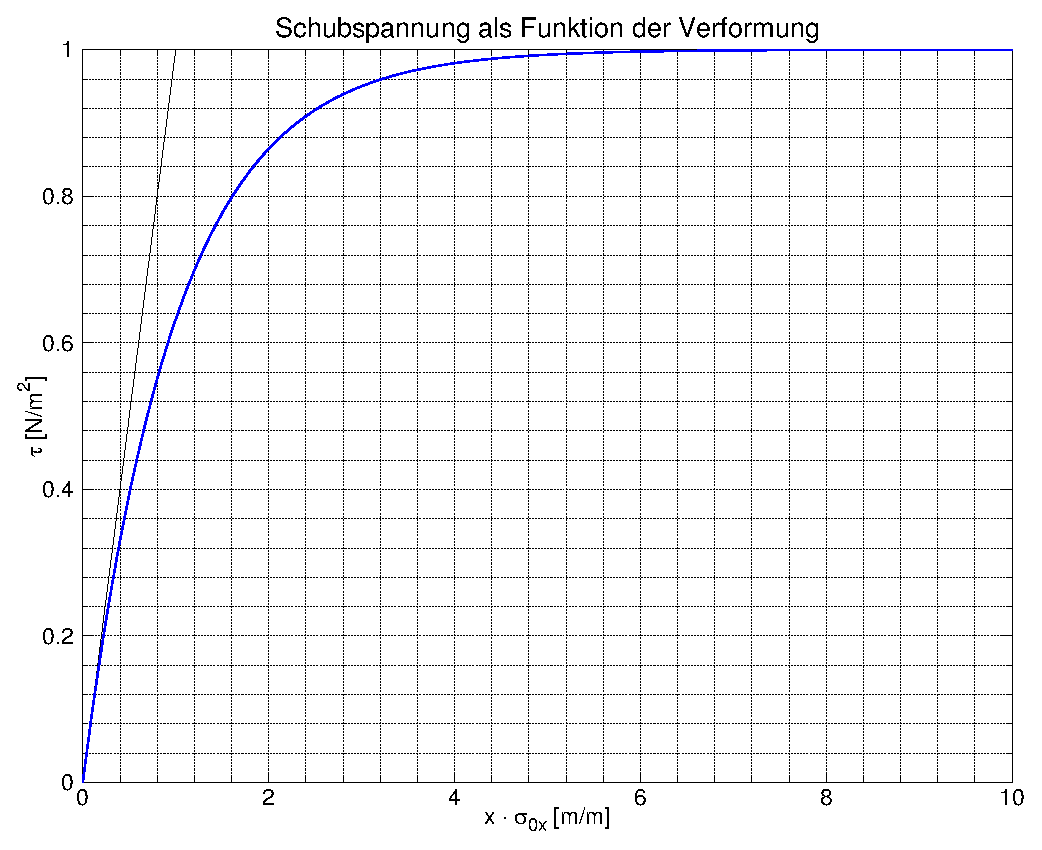
\includegraphics[width=0.5\linewidth]{fig_h900}
\caption{Shear stress distribution as a function of deformation in the one-dimensional LuGre model}
\label{fig:h900}
\end{figure}

\subsubsection{Numerical integration of the LuGre model}
In principle, the linear differential equation for the LuGre model could be solved together with the other equations of the multi-body system. However, this would triple the size of the Jacobian matrix, as the states $\boldsymbol{z}$ for the transition between static friction and dynamic friction would have to be stored for each node in addition to the hydrodynamic pressure $p$. However, since the differential equation of the LuGre model is linear and the static friction states of the individual nodes are independent, the LuGre model was numerically integrated separately from the other equations. The following integration scheme is used for this purpose:
\begin{IEEEeqnarray}{rCl}
\left.\boldsymbol{z}\right\vert_{t} & = & \left[\zeta \,
\left.\dot{\boldsymbol{z}}\right\vert_{t} + \left(1 - \zeta\right) \,
\left.\dot{\boldsymbol{z}}\right\vert_{t - 1}\right] \, \Delta t +
\left.\boldsymbol{z}\right\vert_{t - 1}
\end{IEEEeqnarray}

\begin{description}
\item[$\Delta t$] time step size
\item[$\zeta=0$] explicit Euler method (unstable)
\item[$\zeta=\frac{1}{2}$] trapezoidal rule (second order accurate)
\item[$\zeta=1$] implicit Euler method (first order accurate)
\end{description}

With these assumptions, the following equation for $\dot{\boldsymbol{z}}$ results:
\begin{IEEEeqnarray}{rCl}
\left.\boldsymbol{A}\right\vert_t & = & \left.\kappa\right\vert_t \, \boldsymbol{M}_k^{-2} \,
\boldsymbol{\sigma}_0
\\
\left.\dot{\boldsymbol{z}}\right\vert_{t} & = & \left(\boldsymbol{I} + \zeta \, \Delta t \,
\left.\boldsymbol{A}\right\vert_t\right)^{-1} \, \left\{ \left.\Delta\boldsymbol{U}\right\vert_{t} -
\left.\boldsymbol{A}\right\vert_t \, \left[\left(1 - \zeta\right) \,
\left.\dot{\boldsymbol{z}}\right\vert_{t-1} \, \Delta t +
\left.\boldsymbol{z}\right\vert_{t-1}\right]\right\}
\end{IEEEeqnarray}

\section{Reaction forces}
\subsection{Frictional forces due to fluid friction}
For a Newtonian fluid in laminar flow, the shear stresses $\tau_{xy}$ and $\tau_{yz}$ apply:
\begin{IEEEeqnarray}{rCl}
\tau_{xy} & = & \eta \, \left(\frac{\partial u_x}{\partial y} + \underbrace{\frac{\partial
u_y}{\partial x}}_{\approx 0}\right) \nonumber \\
\tau_{yz} & = & \eta \, \left(\underbrace{\frac{\partial u_y}{\partial z}}_{\approx 0} +
\frac{\partial u_z}{\partial y}\right) \label{eq:h800}
\end{IEEEeqnarray}
As in the derivation of the Reynolds differential equation, the derivatives of the velocity in the circumferential direction and axial direction are neglected compared to the derivative in the radial gap height direction. If equation~\ref{eq:h325} is differentiated versus $y$, the velocity gradients are obtained:
\begin{IEEEeqnarray}{rCl}
\frac{\partial u_x}{\partial y} & = & \frac{1}{\eta} \, \frac{\partial p}{\partial x} \,
\left(y - \frac{h}{2}\right) + \frac{\Delta U_{1x} - \Delta U_{2x}}{h} \nonumber \\
\frac{\partial u_z}{\partial y} & = & \frac{1}{\eta} \, \frac{\partial p}{\partial z} \,
\left(y - \frac{h}{2}\right) + \frac{\Delta U_{1z} - \Delta U_{2z}}{h} \label{eq:h900}
\end{IEEEeqnarray}
Substituting equation~\ref{eq:h900} into equation~\ref{eq:h800} gives the shear stresses at the surface of the components:
\begin{IEEEeqnarray}{rCl}
\left.\tau_{xy}\right\vert_{y=0} & = & - \frac{h}{2} \, \frac{\partial
p}{\partial x} + \eta \, \frac{\Delta U_{1x} - \Delta U_{2x}}{h} \\
\left.\tau_{xy}\right\vert_{y=h} & = & \frac{h}{2} \, \frac{\partial
p}{\partial x} + \eta \, \frac{\Delta U_{1x} - \Delta U_{2x}}{h} \\
\left.\tau_{yz}\right\vert_{y=0} & = & - \frac{h}{2} \, \frac{\partial p}{\partial z} + \eta \,
\frac{\Delta U_{1z} - \Delta U_{2z}}{h} \\
\left.\tau_{yz}\right\vert_{y=h} & = & \frac{h}{2} \, \frac{\partial p}{\partial z} + \eta \,
\frac{\Delta U_{1z} - \Delta U_{2z}}{h}
\end{IEEEeqnarray}
\subsubsection{Micro hydrodynamic effects}
In order to account for micro hydrodynamic effects also the shear stresses must be corrected\cite{PatirCheng1979}. The corrected shear stresses are:
\begin{IEEEeqnarray}{rCl}
\left.\tau_{xy}\right\vert_{y=0} & = & -\phi_{fp_{xy}} \, \frac{h}{2} \, \frac{\partial p}{\partial x} + \eta \, \frac{\Delta U_{1x} - \Delta U_{2x}}{h} \, \left(\phi_f + \phi_{fs_{xy}}\right)\\
\left.\tau_{xy}\right\vert_{y=h} & = & \phi_{fp_{xy}} \, \frac{h}{2} \, \frac{\partial p}{\partial x} + \eta \, \frac{\Delta U_{1x} - \Delta U_{2x}}{h} \, \left(\phi_f - \phi_{fs_{xy}}\right)\\
\left.\tau_{yz}\right\vert_{y=0} & = & -\phi_{fp_{yz}}\,\frac{h}{2} \, \frac{\partial p}{\partial z} + \eta \,
\frac{\Delta U_{1z} - \Delta U_{2z}}{h} \, \left(\phi_f + \phi_{fs_{yz}}\right)\\
\left.\tau_{yz}\right\vert_{y=h} & = & \phi_{fp_{yz}}\,\frac{h}{2} \, \frac{\partial p}{\partial z} + \eta \,\frac{\Delta U_{1z} - \Delta U_{2z}}{h}\,\left(\phi_f - \phi_{fs_{yz}}\right)
\end{IEEEeqnarray}
Where $\phi_{fp_{xy}}$ and $\phi_{fp_{yz}}$ are the shear stress factors due to pressure gradient in $x$ and $z$ direction respectively. $\phi_{fs_{xy}}$ and $\phi_{fs_{yz}}$ are the shear stress factors due to sliding and roughness in $x$ and $z$ direction respectively. $\phi_f$ is the mean shear stress factor which accounts for the change in the base shear stress due to the varying gap height. Those factors are defined as\cite{PatirCheng1979}:
\begin{IEEEeqnarray}{rCl}
\phi_{fp}&=&1 - D\,\exp{\left(-s\,H\right)} \\
\phi_{fp_{xy}}&=&\phi_{fp}\left(H, \gamma_c\right) \\
\phi_{fp_{yz}}&=&\phi_{fp}\left(H, \frac{1}{\gamma_c}\right) \\
\phi_{fs_{xy}}&=&V_{r1}\,\Phi_{fs}\left(H, \gamma_1\right) - V_{r2}\,\Phi_{fs}\left(H, \gamma_2\right) \\
\phi_{fs_{yz}}&=&V_{r1}\,\Phi_{fs}\left(H, \frac{1}{\gamma_1}\right) - V_{r2}\,\Phi_{fs}\left(H, \frac{1}{\gamma_2}\right) \\
\Phi_{fs}&=&A_3\,H^{\alpha_4}\,\exp{\left(-\alpha_5\,H+\alpha_6\,H^2\right)} \\
\phi_f & = & \left\{\begin{array}{rcl} 1 + \frac{0.88}{H^{1.5}} & \text{if} & 0.5 \leq H \leq 5 \\
                                1 + \frac{1}{H^2} & \text{if} & H > 5
             \end{array}\right.
\end{IEEEeqnarray}
The coefficients for $\phi_{fp_{xy}}$ and $\phi_{fp_{yz}}$ must be interpolated from table~\ref{tb:h901} whereas the coefficients for $\Phi_{fs_{xy}}$ and $\Phi_{fs_{yz}}$ must be interpolated from table~\ref{tb:h900}.

\begin{table}
\centering
\caption{Coefficients for the calculation of the shear stress factors $\phi_{fs}$\cite{PatirCheng1979}}
\begin{tabular}{c|c|c|c|c}
\hline
$\gamma_1/\gamma_2$ & $A_3$ & $\alpha_4$ & $\alpha_5$ & $\alpha_6$ \\
\hline
1/9 & 14.1 & 2.45 & 2.30 & 0.10 \\
1/6 & 13.4 & 2.42 & 2.30 & 0.10 \\
1/3 & 12.3 & 2.32 & 2.30 & 0.10 \\
  1 & 11.1 & 2.31 & 2.38 & 0.11 \\
  3 &  9.8 & 2.25 & 2.80 & 0.18 \\
  6 & 10.1 & 2.25 & 2.90 & 0.18 \\
  9 &  8.7 & 2.15 & 2.97 & 0.18
\end{tabular}
\label{tb:h900}
\end{table}

\begin{table}
\centering
\caption{Coefficients for the calculation of the shear stress factors $\phi_{fp}$\cite{PatirCheng1979}}
\begin{tabular}{c|c|c}
\hline
$\gamma_c$ & $D$ & $s$ \\
\hline
1/9 & 1.51 & 0.52 \\
1/6 & 1.51 & 0.54 \\
1/3 & 1.47 & 0.58 \\
  1 & 1.40 & 0.66 \\
  3 & 0.98 & 0.79 \\
  6 & 0.97 & 0.91 \\
  9 & 0.73 & 0.91
\end{tabular}
\label{tb:h901}
\end{table}

\subsection{The mesh moves with the bearing shell}
\label{sec:h350}
The reaction forces on the bearing journal and on the bearing shell result from the integration of the shear stresses and the pressure loads over the surface. The kinematic relationships are shown in Figure~\ref{fig:h800}.

\begin{figure}[htb]
\centering
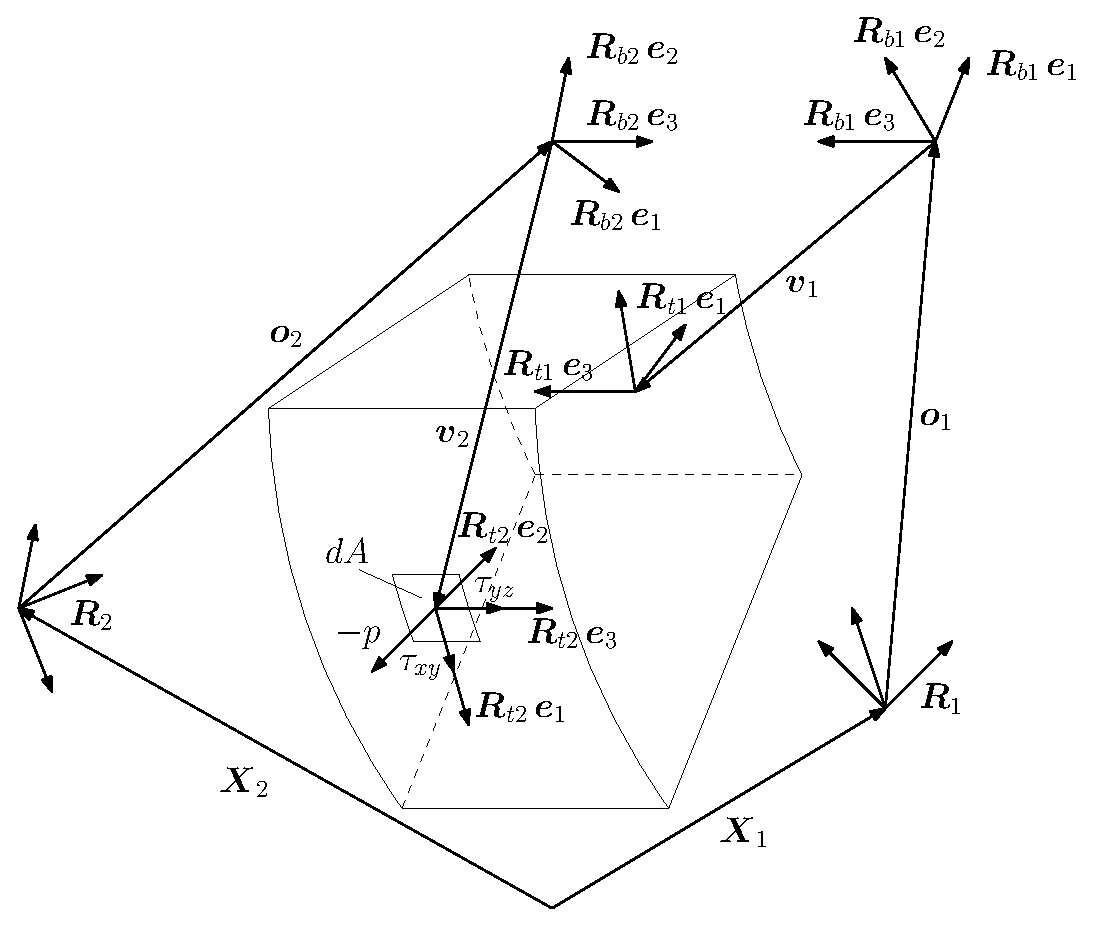
\includegraphics[width=0.5\linewidth]{fig_h800}
\caption{Reaction forces with a mesh on the bearing shell}
\label{fig:h800}
\end{figure}

\subsubsection{Forces on the bearing shell}
\label{sec:h300}
The integration of the reaction forces on the bearing shell is conveniently carried out in the coordinate system of the node of the bearing shell.
\begin{IEEEeqnarray}{rCl}
d\boldsymbol{F}_{2}^{\left(\boldsymbol{R}_2\right)} & = & \boldsymbol{R}_{b2} \, \boldsymbol{R}_{t2}
\,
\begin{pmatrix}
\left.\tau_{xy}\right\vert_{y=0} + \tau_{asp_{xy}} \cr
-\left(p + p_{asp}\right) \cr
\left.\tau_{yz}\right\vert_{y=0} + \tau_{asp_{yz}}
\end{pmatrix}
\, dA_2 \\
d\boldsymbol{M}_2^{\left(\boldsymbol{R}_2\right)} & = & \left\langle \boldsymbol{R}_{b2} \,
\boldsymbol{v}_2 \right\rangle \, d\boldsymbol{F}_2^{\left(\boldsymbol{R}_2\right)} \\
\boldsymbol{F}_2 & = & \boldsymbol{R}_2 \, \int_{A_2}
d\boldsymbol{F}_2^{\left(\boldsymbol{R}_2\right)} \label{eq:h310}
\\
\boldsymbol{M}_2 & = & \left\langle\boldsymbol{R}_2\,\boldsymbol{o}_2\right\rangle \,
\boldsymbol{F}_2 + \boldsymbol{R}_2 \, \int_{A_2} d\boldsymbol{M}_2^{\left(\boldsymbol{R}_2\right)} \label{eq:h311}
\end{IEEEeqnarray}

\subsubsection{Forces on the bearing journal}
\label{sec:h400}
Since the shear stresses due to fluid friction are different on the bearing journal at $y=h$ and on the bearing shell at $y=0$, the reaction forces on both sides must be integrated. The integration of the reaction forces on the bearing journal also takes place in the coordinate system of the bearing shell. In case of an axial movement between journal and shell surface, the projected distance $\lambda$ in equation~\ref{eq:h411} must be considered in the moment equilibrium. This is important, especially for piston to cylinder liner contacts.

\begin{IEEEeqnarray}{rCl}
d\boldsymbol{F}_1^{\left(\boldsymbol{R}_2\right)} & = & \boldsymbol{R}_{b2}\,\boldsymbol{R}_{t2} \,
\begin{pmatrix}
\left.-\tau_{xy}\right\vert_{y=h} -\tau_{asp_{xy}} \cr
p + p_{asp} \cr
\left.-\tau_{yz}\right\vert_{y=h} - \tau_{asp_{yz}}
\end{pmatrix} \, dA_2 \\
d\boldsymbol{M}_1^{\left(\boldsymbol{R}_2\right)} & = & \left\langle \boldsymbol{R}_{b2} \, \boldsymbol{v}_2
\right\rangle \, d\boldsymbol{F}_1^{\left(\boldsymbol{R}_2\right)} \\
\boldsymbol{F}_1 & = & \boldsymbol{R}_2 \, \int_{A_2} d\boldsymbol{F}_1^{\left(\boldsymbol{R}_2\right)} \label{eq:h410} \\
\boldsymbol{M}_1 & = & \left\langle \boldsymbol{R}_1 \, \left(\boldsymbol{o}_1 + \boldsymbol{R}_{b1} \, \boldsymbol{e}_3 \, \lambda \right) \right\rangle \,
\boldsymbol{F}_1 + \boldsymbol{R}_2\,\int_{A_2} d\boldsymbol{M}_1^{\left(\boldsymbol{R}_2\right)} \label{eq:h411} \\
\lambda & = & -\frac{\boldsymbol{e}_3^T\,\boldsymbol{R}_{b2}^T\,\left[\boldsymbol{R}_2^T\,\left(\boldsymbol{X}_1 + \boldsymbol{R}_1\,\boldsymbol{o}_1 - \boldsymbol{X}_2\right) - \boldsymbol{o}_2\right]}{\boldsymbol{e}_3^T\,\boldsymbol{R}_{b2}^T\,\boldsymbol{R}_2^T\,\boldsymbol{R}_1\,\boldsymbol{R}_{b1}\,\boldsymbol{e}_3}
\end{IEEEeqnarray}

\subsection{The mesh moves with the bearing journal}
In this case, the same procedure is applied as described in section~\ref{sec:h350}.
\subsubsection{Forces on the bearing journal}
The following applies to the forces on the bearing journal:
\begin{IEEEeqnarray}{rCl}
d\boldsymbol{F}_1^{\left(\boldsymbol{R}_1\right)} & = & \boldsymbol{R}_{b1} \, \boldsymbol{R}_{t1}
\,
\begin{pmatrix}
-\left.\tau_{xy}\right\vert_{y=h} - \tau_{asp_{xy}} \cr
p + p_{asp} \cr
-\left.\tau_{yz}\right\vert_{y=h} - \tau_{asp_{yz}}
\end{pmatrix}
\, dA_1 \\
d\boldsymbol{M}_1^{\left(\boldsymbol{R}_1\right)} & = & \left\langle \boldsymbol{R}_{b1} \,
\boldsymbol{v}_1 \right\rangle \, d\boldsymbol{F}_1^{\left(\boldsymbol{R}_1\right)} \\
\boldsymbol{F}_1 & = & \boldsymbol{R}_1 \, \int_{A_1}
d\boldsymbol{F}_1^{\left(\boldsymbol{R}_1\right)} \label{eq:h420}
\\
\boldsymbol{M}_1 & = & \left\langle \boldsymbol{R}_1 \, \boldsymbol{o}_1
\right\rangle \, \boldsymbol{F}_{1} + \boldsymbol{R}_1 \, \int_{A_1}
d\boldsymbol{M}_1^{\left(\boldsymbol{R}_1\right)} \label{eq:h421}
\end{IEEEeqnarray}

\subsubsection{Forces on the bearing shell}
Also the forces at the bearing shell are calculated analogous to section~\ref{sec:h400}.
\begin{IEEEeqnarray}{rCl}
d\boldsymbol{F}_2^{\left(\boldsymbol{R}_1\right)} & = & \boldsymbol{R}_{b1} \, \boldsymbol{R}_{t1} \,
\begin{pmatrix}
\left.\tau_{xy}\right\vert_{y=0} + \tau_{asp_{xy}} \cr
-p - p_{asp} \cr
\left.\tau_{yz}\right\vert_{y=0} + \tau_{asp_{yz}}
\end{pmatrix}
\, dA_1 \\
d\boldsymbol{M}_2^{\left(\boldsymbol{R}_1\right)} & = & \left\langle \boldsymbol{R}_{b1} \, \boldsymbol{v}_{1} \, \right\rangle \, d\boldsymbol{F}_2^{\left(\boldsymbol{R}_1\right)} \\
\boldsymbol{F}_2 & = & \boldsymbol{R}_1 \, \int_{A_1} d\boldsymbol{F}_2^{\left(\boldsymbol{R}_1\right)} \label{eq:h430} \\
\boldsymbol{M}_2 & = & \left\langle \boldsymbol{R}_2 \, \left(\boldsymbol{o}_2 + \boldsymbol{R}_{b2} \, \boldsymbol{e}_3 \, \lambda \right) \right\rangle \,
\boldsymbol{F}_2 + \boldsymbol{R}_1 \, \int_{A_1} d\boldsymbol{M}_2^{\left(\boldsymbol{R}_1\right)} \label{eq:h431} \\
\lambda & = & \frac{\boldsymbol{e}_3^T\,\boldsymbol{R}_{b1}^T\,\left[\boldsymbol{R}_1^T\left(\boldsymbol{X}_1 - \boldsymbol{X}_2 - \boldsymbol{R}_2\,\boldsymbol{o}_2\right) + \boldsymbol{o}_1\right]}{\boldsymbol{e}_3^T\,\boldsymbol{R}_{b1}^T\,\boldsymbol{R}_1^T\,\boldsymbol{R}_2\,\boldsymbol{R}_{b2}\,\boldsymbol{e}_3}
\end{IEEEeqnarray}

\subsection{Determination of frictional losses}
Theoretically, the frictional losses could also be determined from the bearing reaction forces. However, it is not possible to separate dry friction from fluid friction and it is difficult to separate the dissipative components from the conservative components. For this reason, the friction power was determined independently of the reaction forces.
\begin{IEEEeqnarray}{rCl}
P_f & = & -\int_A \left[\left(\Delta U_{1x} - \Delta U_{2x}\right)\, \left.\tau_{xy}\right\vert_{y=0} + \left(\Delta U_{1z} - \Delta U_{2z}\right)\,
\left.\tau_{yz}\right\vert_{y=0} \right]\,dA \label{eq:h500} \\
P_{asp} & = & -\int_A \left[\left(\Delta U_{1x} - \Delta U_{2x}\right)\, \tau_{asp_{xy}} + \left(\Delta U_{1z} - \Delta U_{2z}\right)\,
\tau_{asp_{yz}}\right]\,dA \label{eq:h501}
\end{IEEEeqnarray}
The negative sign in equation~\ref{eq:h500} and equation~\ref{eq:h501} follows the convention that kinetic energy losses are denoted as negative.
\begin{description}
\item[$P_f$] Frictional losses due to fluid friction
\item[$P_{asp}$] Frictional losses due to dry friction
\end{description}

\section{Alternative solution of the incompressible Reynolds differential equation using the
finite element method}
The discretization chosen in section~\ref{sec:h150} using finite differences was based on an orthogonal grid. This is completely sufficient for simple geometries such as a cylindrical plain bearing without lubrication grooves. Even a rectangular lubrication groove can still be captured accurately thanks to the variable grid spacing. In the case of a circular lubricating oil bore, however, the method is very inefficient, as a very fine grid is required for accurate resolution of the circular edge, which extends over the entire bearing surface due to the orthogonal grid lines in the circumferential direction and in the axial direction. Using the finite element method, however, makes it much easier to handle complex geometries. The general procedure for the discretization of partial differential equations in this section is essentially based on \cite{BATHE2016}.

\subsection{The weak formulation of the Reynolds differential equation}
The starting point for the finite element formulation is the incompressible Reynolds differential equation. In equation~\ref{eq:hfe_100} it was assumed that the radial velocity of the bearing journal is small compared to the circumferential velocity. This results in the frequently encountered simplification $\frac{\partial}{\partial x}\left(\frac{\Delta U_{1x} + \Delta U_{2x}}{2} \, h\right)\approx \frac{\Delta U_{1x} + \Delta U_{2x}}{2} \, \frac{\partial h}{\partial x}$.

\begin{IEEEeqnarray}{rCl}
\label{eq:hfe_100}
\frac{\partial}{\partial x} \left(h^3 \, \frac{\partial p}{\partial x} \right) +
\frac{\partial}{\partial z} \left(h^3 \, \frac{\partial p}{\partial z}\right) & = & 12 \, \eta
\left[\frac{\partial h}{\partial t} + \frac{\Delta U_{1x} + \Delta U_{2x}}{2} \,
\frac{\partial h}{\partial x} + \frac{\Delta U_{1z} + \Delta U_{2z}}{2} \, \frac{\partial
h}{\partial z}\right]
\end{IEEEeqnarray}

Equation~\ref{eq:hfe_100} is multiplied by the test function $\bar{p}$ and integrated over the entire solution domain.

\begin{IEEEeqnarray}{lCl}
\int_{A} \left\{ \bar{p} \, \left[\frac{\partial}{\partial x} \left(h^3 \, \frac{\partial
p}{\partial x} \right) + \frac{\partial}{\partial z} \left(h^3 \, \frac{\partial p}{\partial
z}\right)\right] \right. \nonumber \\
\left. - 12 \, \eta \, \bar{p} \, \left(\frac{\partial h}{\partial t}
+ \frac{\Delta U_{1x} + \Delta U_{2x}}{2} \, \frac{\partial h}{\partial x} + \frac{\Delta U_{1z} + \Delta
U_{2z}}{2} \, \frac{\partial h}{\partial z} \right) \right\} \, dA & = & 0
\end{IEEEeqnarray}

The aim is to eliminate the second derivatives from the partial differential equation. The advantage of this is that it allows lower-order shape~functions to be used\cite{BATHE2016}. For this purpose, the partial differential equation is transformed using Gauss's integral theorem and the chain rule of differentiation so that only first derivatives appear\cite{BATHE2016}. This follows from the chain rule of differentiation:

\begin{IEEEeqnarray}{lCl}
\int_{A} \left\{ \frac{\partial}{\partial x} \left(\bar{p} \, h^3 \, \frac{\partial
p}{\partial x}\right) - \frac{\partial \bar{p}}{\partial x} \, h^3 \, \frac{\partial p}{\partial x}
+ \frac{\partial}{\partial z} \left(\bar{p} \, h^3 \, \frac{\partial p}{\partial z} \right) -
\frac{\partial \bar{p}}{\partial z} \, h^3 \, \frac{\partial p}{\partial z} \right. \nonumber \\
\left.- 12 \, \eta \, \bar{p} \left(\frac{\partial h}{\partial t} + \frac{\Delta U_{1x} + \Delta
U_{2x}}{2} \, \frac{\partial h}{\partial x} +
\frac{\Delta U_{1z} + \Delta U_{2z}}{2} \, \frac{\partial h}{\partial z}\right) \, \right\} \, dA &
= & 0
\end{IEEEeqnarray}

The Gaussian integral theorem reads:

\begin{IEEEeqnarray}{rCl}
\int_{A} \left(\frac{\partial Q}{\partial x} - \frac{\partial P}{\partial z}\right) \, dA & = &
\oint_{R} P \, dx + Q \, dz
\end{IEEEeqnarray}

After applying Gauss's integral theorem, the following results:

\begin{IEEEeqnarray}{lCl}
\label{eq:hfe_150}
\int_{A} \left(\frac{\partial \bar{p}}{\partial x} \, h^3 \, \frac{\partial p}{\partial x} +
\frac{\partial \bar{p}}{\partial z} \, h^3 \, \frac{\partial p}{\partial z}\right) \, dA \nonumber
\\
+ 12 \, \eta \int_{A} \bar{p} \left(\frac{\partial h}{\partial t} + \frac{\Delta U_{1x} +
\Delta U_{2x}}{2} \, \frac{\partial h}{\partial x} + \frac{\Delta U_{1z} + \Delta U_{2z}}{2}
\, \frac{\partial h}{\partial z}\right)\,dA \nonumber \\
= \oint_{R} -\bar{p} \, h^3 \, \frac{\partial p}{\partial z} \, dx + \bar{p} \, h^3 \,
\frac{\partial p}{\partial x} \, dz
\end{IEEEeqnarray}

The boundary $R$ of the solution domain can now be divided into two areas:

\begin{description}
\item[$R_p$] edge at which the pressure $p$ is prescribed and the pressure gradient can be freely adjusted. Therefore, $\left.\bar{p}\right\vert_{R_p}=0$ applies to this boundary
\item[$R_g$] boundary at which the pressure gradient $\frac{\partial p}{\partial x}$ or $\frac{\partial
p}{\partial z}$ is prescribed and the pressure $p$ can be freely adjusted.
\end{description}

With these assumptions, the integrals over the boundaries of the bearing surface can be transformed as follows:

\begin{IEEEeqnarray}{lCl}
\label{eq:hfe_175}
\oint_{R} -\bar{p} \, h^3 \, \frac{\partial p}{\partial z} \, dx + \bar{p} \, h^3 \, \frac{\partial
p}{\partial x} \, dz \nonumber \\
= \underbrace{-\oint_{R_p} \bar{p} \, h^3 \, \frac{\partial p}{\partial z} \, dx}_{=0} - \oint_{R_g}
\bar{p} \, h^3 \left.\frac{\partial p}{\partial z}\right\vert_g \, dx \nonumber \\
+\underbrace{\oint_{R_p} \bar{p} \, h^3 \, \frac{\partial p}{\partial x} \, dz}_{=0} + \oint_{R_g}
\bar{p} \, h^3 \, \left.\frac{\partial p}{\partial x}\right\vert_g \, dz
\end{IEEEeqnarray}

\subsection{Discretization using isoparametric finite elements}
According to \cite{BATHE2016}, the unknown pressures $p$ and the test function $\bar{p}$ inside an element are interpolated using shape or interpolation functions $\boldsymbol{N}$ from the pressures $\boldsymbol{p}_e$ in the nodes of an element. The pressure gradients $\frac{\partial p}{\partial x}$ and $\frac{\partial p}{\partial z}$ are calculated using the derivatives $\boldsymbol{B}_1$ and $\boldsymbol{B}_2$ of those shape functions. The following applies:

\begin{IEEEeqnarray}{rCl}
\label{eq:hfe_200}
p & = & \boldsymbol{N} \, \hat{\boldsymbol{p}}_e \\
\bar{p} & = & \boldsymbol{N} \, \bar{\hat{\boldsymbol{p}}}_e \nonumber \\
& = & \bar{\hat{\boldsymbol{p}}}_e^T \, \boldsymbol{N}^T \\
\frac{\partial p}{\partial x} & = & \boldsymbol{B}_1 \, \hat{\boldsymbol{p}}_e \\
\frac{\partial \bar{p}}{\partial x} & = & \boldsymbol{B}_1 \, \bar{\hat{\boldsymbol{p}}}_e
\nonumber \\
& = & \hat{\bar{\boldsymbol{p}}}_e^T \, \boldsymbol{B}_1^T \\
\frac{\partial p}{\partial z} & = & \boldsymbol{B}_2 \, \hat{\boldsymbol{p}}_e \\
\frac{\partial \bar{p}}{\partial z} & = & \boldsymbol{B}_2 \, \bar{\hat{\boldsymbol{p}}}_e \nonumber
\\
& = & \bar{\hat{\boldsymbol{p}}}_e^T \, \boldsymbol{B}_2^T
\end{IEEEeqnarray}


\begin{IEEEeqnarray}{rCl}
h & = & \boldsymbol{N} \, \hat{\boldsymbol{h}}_e \\
\frac{\partial h}{\partial t} & = & \boldsymbol{N} \, \frac{\partial
\hat{\boldsymbol{h}}_e}{\partial t} \\
\frac{\partial h}{\partial x} & = & \boldsymbol{B}_1 \, \hat{\boldsymbol{h}}_e \\
\frac{\partial h}{\partial z} & = & \boldsymbol{B}_2 \, \hat{\boldsymbol{h}}_e \\
\Delta U_{1x} & = & \boldsymbol{N} \, \Delta\hat{\boldsymbol{U}}_{1x_e} \\
\Delta U_{2x} & = & \boldsymbol{N} \, \Delta\hat{\boldsymbol{U}}_{2x_e} \\
\Delta U_{1z} & = & \boldsymbol{N} \, \Delta\hat{\boldsymbol{U}}_{1z_e} \\
\Delta U_{2z} & = & \boldsymbol{N} \, \Delta\hat{\boldsymbol{U}}_{2z_e} \\
\left.\frac{\partial p}{\partial x}\right\vert_{g_e} & = & \boldsymbol{N} \, \left.\frac{\partial
\hat{\boldsymbol{p}}}{\partial x}\right\vert_{g_e} \\
\label{eq:hfe_300}
\left.\frac{\partial p}{\partial z}\right\vert_{g_e} & = & \boldsymbol{N} \, \left.\frac{\partial
\hat{\boldsymbol{p}}}{\partial z}\right\vert_{g_e}
\end{IEEEeqnarray}

\begin{description}
\item[$\hat{\boldsymbol{p}}_e$] Pressure in the node of the element~$e$
\item[$\bar{\hat{\boldsymbol{p}}}_e$] Test function in the nodes of the element~$e$
\item[$\hat{\boldsymbol{h}}_e$] radial gap height in the nodes of the element~$e$
\item[$\Delta\hat{\boldsymbol{U}}_{1x_e}$] relative velocity of the bearing journal in $x$-direction in the nodes of the element~$e$.
\item[$\Delta\hat{\boldsymbol{U}}_{1z_e}$] relative velocity of the bearing journal in $z$-direction in the nodes of the element~$e$
\item[$\left.\frac{\partial \hat{\boldsymbol{p}}}{\partial x}\right\vert_{g_e}$] prescribed pressure gradient in $x$-direction in the nodes of the element~$e$
\item[$\left.\frac{\partial \hat{\boldsymbol{p}}}{\partial z}\right\vert_{g_e}$] prescribed pressure gradient in $z$-direction in the nodes of the element~$e$
\item[$\boldsymbol{N}$] Matrix for interpolating the pressures within the element~$e$
\item[$\boldsymbol{B}_1$, $\boldsymbol{B}_2$] Matrices for interpolating the pressure gradients in the $x$-
and $z$-direction
\end{description}
The matrices $\boldsymbol{N}$ and $\boldsymbol{B}$ depend on the selected element type. Isoparametric elements with four or nine nodes from \cite{BATHE2016} were used. In contrast to finite difference discretization, these elements can be used to approximate complex geometries without additional implementation effort. For example, the mesh can be adapted to circular lubricating oil holes and these can thus be approximated very accurately.

\subsubsection{An isoparametric element with four nodes}
The following element matrices for the four-node element result from the shape~functions from \cite{BATHE2016}:
\begin{IEEEeqnarray}{rCl}
h_1 & = & \frac{\left( r+1\right) \,\left( s+1\right)}{4} \\
h_2 & = & \frac{\left( 1-r\right) \,\left( s+1\right)}{4} \\
h_3 & = & \frac{\left( 1-r\right) \,\left( 1-s\right)}{4} \\
h_4 & = & \frac{\left( r+1\right) \,\left( 1-s\right)}{4} \\
\boldsymbol{N} & = &
\begin{pmatrix}
h_1 & h_2 & h_3 & h_4
\end{pmatrix}
\end{IEEEeqnarray}

\subsubsection{An isoparametric element with nine nodes}
The shape functions for the nine-node element are an extension of the shape functions of the four-node element and also originate from \cite{BATHE2016}.
\begin{IEEEeqnarray}{rCl}
h_9 & = & \left( 1-{r}^{2}\right) \,\left( 1-{s}^{2}\right) \\
h_5 & = & \frac{\left( 1-{r}^{2}\right) \,\left( s+1\right) }{2}-\frac{h_9}{2} \\
h_6 & = & \frac{\left( 1-r\right) \,\left( 1-{s}^{2}\right) }{2}-\frac{h_9}{2} \\
h_7 & = & \frac{\left( 1-{r}^{2}\right) \,\left( 1-s\right) }{2}-\frac{h_9}{2} \\
h_8 & = & \frac{\left( r+1\right) \,\left( 1-{s}^{2}\right) }{2}-\frac{h_9}{2} \\
h_1 & = & \frac{\left( r+1\right) \,\left( s+1\right)
}{4}-\frac{h_9}{4}-\frac{h_8}{2}-\frac{h_5}{2} \\
h_2 & = & \frac{\left( 1-r\right) \,\left( s+1\right) }{4}-\frac{h_9}{4}-\frac{h_6}{2}-\frac{h_5}{2}
\\
h_3 & = & \frac{\left( 1-r\right) \,\left( 1-s\right)}{4}-\frac{h_9}{4}-\frac{h_7}{2}-\frac{h_6}{2}
\\
h_4 & = & \frac{\left( r+1\right) \,\left( 1-s\right)
}{4}-\frac{h_9}{4}-\frac{h_8}{2}-\frac{h_7}{2} \\
\boldsymbol{N} & = &
\begin{pmatrix}
h_1 & h_2 & h_3 & h_4 & h_5 & h_6 & h_7 & h_8 & h_9
\end{pmatrix}
\end{IEEEeqnarray}

\subsubsection{Determination of the distortion interpolation matrix}
The following applies to all two-dimensional isoparametric elements
\begin{IEEEeqnarray}{rCl}
x\left(r,\, s\right) & = & \boldsymbol{N} \, \hat{\boldsymbol{x}}_e \\
z\left(r,\,s\right) & = & \boldsymbol{N} \, \hat{\boldsymbol{z}}_e \\
\boldsymbol{J} &=& \begin{pmatrix}
\frac{\partial x}{\partial r} & \frac{\partial z}{\partial r} \cr
\frac{\partial x}{\partial s} & \frac{\partial z}{\partial s}
\end{pmatrix} \\
\boldsymbol{B} & = & \begin{pmatrix}
\boldsymbol{B}_1 \cr
\boldsymbol{B}_2
\end{pmatrix} \nonumber \\
& = & \boldsymbol{J}^{-1} \, \begin{pmatrix}
\frac{\partial \boldsymbol{N}}{\partial r} \cr
\frac{\partial \boldsymbol{N}}{\partial s}
\end{pmatrix}
\end{IEEEeqnarray}

\begin{description}
\item[$h_1$, $h_2$, $\hdots$] shape functions
\item[$\boldsymbol{J}$] Jacobian matrix of the element
\item[$\hat{\boldsymbol{x}}_e$] $x$-coordinates of the nodes in the unrolled bearing surface
\item[$\hat{\boldsymbol{z}}_e$] $z$-coordinates of the nodes in the unrolled bearing surface
\end{description}

\subsubsection{Structure of the element matrices}
Substituting equation~\ref{eq:hfe_200} to equation~\ref{eq:hfe_300} and equation~\ref{eq:hfe_175} into equation~\ref{eq:hfe_150}, yields:
\begin{IEEEeqnarray}{lCl}
\sum_{e=1}^{N_e} \left\{\bar{\hat{\boldsymbol{p}}}_{e}^T \, \underbrace{\left[\int_{A_e}
\left(\boldsymbol{N} \, \hat{\boldsymbol{h}}_e\right)^3 \, \left( \boldsymbol{B}_1^T \, \boldsymbol{B}_1 +
\boldsymbol{B}_2^T
\,
\boldsymbol{B}_2\right)\,dA_e\right]}_{\boldsymbol{K}_e}\, \hat{\boldsymbol{p}}_{e} \right.
\nonumber
\\
\left. + \bar{\hat{\boldsymbol{p}}}_e^T \, \underbrace{\left[\int_{A_e} 12\, \eta \,
\boldsymbol{N}^T \, \boldsymbol{N} \, \left(\frac{\partial \hat{\boldsymbol{h}}_e}{\partial t} +
\frac{\Delta\hat{\boldsymbol{U}}_{1x_e} + \Delta\hat{\boldsymbol{U}}_{2x_e}}{2} \,
\boldsymbol{B}_1 \, \hat{\boldsymbol{h}}_e + \frac{\Delta\hat{\boldsymbol{U}}_{1z_e} +
\Delta\hat{\boldsymbol{U}}_{2z_e}}{2} \,
\boldsymbol{B}_2 \, \hat{\boldsymbol{h}}_e \right)\,dA\right]}_{-\boldsymbol{R}_e}\right\} \nonumber
\nonumber \\
= \sum_{e=1}^{N_e} \left\{\bar{\hat{\boldsymbol{p}}}_e^T \underbrace{\left[\oint_{R_{g_e}}
\boldsymbol{N}^T \, \boldsymbol{N} \, \left(\boldsymbol{N} \, \hat{\boldsymbol{h}}_e\right)^3 \, \left.\frac{\partial
\hat{\boldsymbol{p}}}{\partial x}\right\vert_{g_e} \, dz - \oint_{R_{g_e}} \boldsymbol{N}^T \,
\boldsymbol{N} \, \left(\boldsymbol{N} \, \hat{\boldsymbol{h}}_e\right)^3 \, \left.\frac{\partial
\hat{\boldsymbol{p}}}{\partial z}\right\vert_{g_e} \, dx\right]}_{\boldsymbol{G}_e}\right\}
\label{eq:hfe_400}
\end{IEEEeqnarray}

The element matrices $\boldsymbol{K}_e$, $\boldsymbol{R}_e$ and $\boldsymbol{G}_e$ are obtained for isoparametric elements by numerical integration over the natural coordinates $r$ and $s$. For the surface integrals $dA=\det{\boldsymbol{J}} \, dr \, ds$.

\begin{IEEEeqnarray}{rCl}
\boldsymbol{K}_e & = & \int_{r=-1}^{1}\int_{s=-1}^{1}
\left(\boldsymbol{N} \, \hat{\boldsymbol{h}}_e\right)^3 \, \left(\boldsymbol{B}_1^T \,
\boldsymbol{B}_1 + \boldsymbol{B}_2^T \, \boldsymbol{B}_2\right) \, \det{\boldsymbol{J}} \, dr \, ds
\\
\boldsymbol{R}_e & = & -\int_{r=-1}^{1}\int_{s=-1}^{1} 12 \, \eta \, \boldsymbol{N}^T \,
\boldsymbol{N} \left(\frac{\Delta\hat{\boldsymbol{U}}_{1x_e} + \Delta\hat{\boldsymbol{U}}_{2x_e}}{2}
\boldsymbol{B}_1 \, \hat{\boldsymbol{h}}_{e} \right. \nonumber \\
& & \left.+\frac{\Delta\hat{\boldsymbol{U}}_{1z_e} + \Delta\hat{\boldsymbol{U}}_{2z_e}}{2}
\boldsymbol{B}_2 \, \hat{\boldsymbol{h}}_{e} +
\frac{\partial \hat{\boldsymbol{h}}_e}{\partial t} \right)\,\det{\boldsymbol{J}}\,dr\,ds \\
\label{eq:hfe_500}
\boldsymbol{G}_e & = & \alpha_1 \, \int_{r=-1}^{1} \left\{\boldsymbol{N}^T \, \boldsymbol{N} \,
\left(\boldsymbol{N} \, \hat{\boldsymbol{h}}_e \right)^3 \, \left[\left.\frac{\partial
\hat{\boldsymbol{p}}}{\partial x}\right\vert_{g_e} \, \frac{\partial \boldsymbol{N}}{\partial r} \,
\hat{\boldsymbol{z}}_{e}\left. - \left.\frac{\partial \hat{\boldsymbol{p}}}{\partial
z}\right\vert_{e} \, \frac{\partial \boldsymbol{N}}{\partial r} \,
\hat{\boldsymbol{x}}_e\right]\right\}\right\vert_{s=-1} \, dr \nonumber \\
&  & + \alpha_2 \, \int_{s=-1}^{1} \left\{\boldsymbol{N}^T \, \boldsymbol{N} \,
\left(\boldsymbol{N} \, \hat{\boldsymbol{h}}_e \right)^3 \, \left[\left.\frac{\partial
\hat{\boldsymbol{p}}}{\partial x}\right\vert_{g_e} \, \frac{\partial \boldsymbol{N}}{\partial s} \,
\hat{\boldsymbol{z}}_{e}\left. - \left.\frac{\partial \hat{\boldsymbol{p}}}{\partial
z}\right\vert_{e} \, \frac{\partial \boldsymbol{N}}{\partial s} \,
\hat{\boldsymbol{x}}_e\right]\right\}\right\vert_{r=-1} \, ds \nonumber \\
& & + \alpha_3 \, \int_{r=-1}^{1} \left\{\boldsymbol{N}^T \, \boldsymbol{N} \,
\left(\boldsymbol{N} \, \hat{\boldsymbol{h}}_e \right)^3 \, \left[\left.\frac{\partial
\hat{\boldsymbol{p}}}{\partial x}\right\vert_{g_e} \, \frac{\partial \boldsymbol{N}}{\partial r} \,
\hat{\boldsymbol{z}}_{e}\left. - \left.\frac{\partial \hat{\boldsymbol{p}}}{\partial
z}\right\vert_{e} \, \frac{\partial \boldsymbol{N}}{\partial r} \,
\hat{\boldsymbol{x}}_e\right]\right\}\right\vert_{s=1} \, dr \nonumber \\
&  & + \alpha_4 \, \int_{s=-1}^{1} \left\{\boldsymbol{N}^T \, \boldsymbol{N} \,
\left(\boldsymbol{N} \, \hat{\boldsymbol{h}}_e \right)^3 \, \left[\left.\frac{\partial
\hat{\boldsymbol{p}}}{\partial x}\right\vert_{g_e} \, \frac{\partial \boldsymbol{N}}{\partial s} \,
\hat{\boldsymbol{z}}_{e}\left. - \left.\frac{\partial \hat{\boldsymbol{p}}}{\partial
z}\right\vert_{e} \, \frac{\partial \boldsymbol{N}}{\partial s} \,
\hat{\boldsymbol{x}}_e\right]\right\}\right\vert_{r=1} \, ds
\end{IEEEeqnarray}

In equation~\ref{eq:hfe_500} the following rule was used for the evaluation of the second type of curve integrals:
\begin{IEEEeqnarray}{lCl}
\oint_{R} P\left(x(t), \, y(t)\right) \, dx + Q\left(x(t), \, y(t)\right) \, dy \nonumber \\
= \int_a^b \left( P\left(x(t), \, y(t)\right) \, \frac{\partial x}{\partial t} + Q\left(x(t), \, y(t)\right) \,
\frac{\partial y}{\partial t}\right) \, dt
\end{IEEEeqnarray}

\begin{description}
\item[$\alpha_1$, $\alpha_2$, $\hdots$] This is a constant which is always equal to one if a boundary condition for the pressure gradient $\left.\frac{\partial p}{\partial x}\right\vert_{g_e}$ or $\left.\frac{\partial p}{\partial z}\right\vert_{g_e}$ is specified at the corresponding edge of the element. Otherwise, $\alpha$ is zero.
\end{description}

\paragraph{Numerical integration of the element matrices}
The numerical integration of the element matrices is carried out using the Gauss Legendre Quadrature. The integration points and the weighting factors were taken from \cite{BATHE2016}. For an undistorted element with four nodes, a single Gaussian point is sufficient to obtain accurate results, and for an undistorted element with nine nodes, four Gaussian points are sufficient.

\subsection{Structure of the system of linear equations}
The system of linear equations is formally constructed using the Boolean matrices $\boldsymbol{T}_e$. However, an index table is used internally in the program which assigns the corresponding global degrees of freedom to the individual nodes.

\begin{IEEEeqnarray}{rCl}
\hat{\boldsymbol{p}}_e & = & \boldsymbol{T}_e \, \hat{\boldsymbol{p}} \label{eq:hfe_600} \\
\bar{\hat{\boldsymbol{p}}}_e & = & \boldsymbol{T}_e \, \bar{\hat{\boldsymbol{p}}}
\label{eq:hfe_601} \\
\bar{\hat{\boldsymbol{p}}}_e^T & = & \bar{\hat{\boldsymbol{p}}}^T \, \boldsymbol{T}_e^T
\label{eq:hfe_602}
\end{IEEEeqnarray}

\begin{description}
\item[$\boldsymbol{T}_e$] Boolean matrix for the element~$e$ which contains the local degrees of freedom
$\hat{\boldsymbol{p}}_e$ to the corresponding global degrees of freedom $\hat{\boldsymbol{p}}$
\item[$\hat{\boldsymbol{p}}$] Global vector of pressures of the finite element system
\item[$\bar{\hat{\boldsymbol{p}}}$] Global vector of test functions of the finite element system
\end{description}
If the expressions from equation~\ref{eq:hfe_600} to equation~\ref{eq:hfe_602} are inserted into equation~\ref{eq:hfe_400}, the global equations for the hydrodynamic pressures in the nodes are obtained.
\begin{IEEEeqnarray}{rCl}
\boldsymbol{K} & = & \sum_{e=1}^{N_e} \boldsymbol{T}_e^T \, \boldsymbol{K}_e \, \boldsymbol{T}_e \\
\boldsymbol{R} & = & \sum_{e=1}^{N_e} \boldsymbol{T}_e^T \, \boldsymbol{R}_e \\
\boldsymbol{G} & = & \sum_{e=1}^{N_e} \boldsymbol{T}_e^T \, \boldsymbol{G}_e \\
\bar{\hat{\boldsymbol{p}}}^T \, \boldsymbol{K} \, \hat{\boldsymbol{p}} & = &
\bar{\hat{\boldsymbol{p}}}^T \, \left(\boldsymbol{R} + \boldsymbol{G}\right) \label{eq:hfe_700}
\end{IEEEeqnarray}

\subsection{Implementation of Dirichlet boundary conditions}
The hydrodynamic pressures in the nodes $\hat{\boldsymbol{p}}$ are now divided into the unknown pressures $\check{\boldsymbol{p}}_1$ and the pressures $\check{\boldsymbol{p}}_2$ known a priori from the boundary conditions. This is done formally using the Boolean matrices $\check{\boldsymbol{T}}_1$ and $\check{\boldsymbol{T}}_2$. However, index tables can be used internally in the program.
\begin{IEEEeqnarray}{rCl}
\hat{\boldsymbol{p}} & = & \check{\boldsymbol{T}}_1 \, \check{\boldsymbol{p}}_1 +
\check{\boldsymbol{T}}_2 \, \check{\boldsymbol{p}}_2 \label{eq:hfe_800} \\
\bar{\hat{\boldsymbol{p}}} & = & \check{\boldsymbol{T}}_1 \, \bar{\check{\boldsymbol{p}}}_1 +
\check{\boldsymbol{T}}_2 \, \bar{\check{\boldsymbol{p}}}_2 \label{eq:hfe_801}
\end{IEEEeqnarray}
The following condition applies to these Boolean matrices:
\begin{IEEEeqnarray}{rCl}
\check{\boldsymbol{T}}_1^T \, \check{\boldsymbol{T}}_2 & = & \boldsymbol{0}
\end{IEEEeqnarray}
Substituting equation~\ref{eq:hfe_800} to \ref{eq:hfe_801} into equation~\ref{eq:hfe_700} yields:
\begin{IEEEeqnarray}{l}
\bar{\check{\boldsymbol{p}}}_1^T \, \check{\boldsymbol{T}}_1^T \, \boldsymbol{K} \,
\check{\boldsymbol{T}}_1 \, \check{\boldsymbol{p}}_1 + \check{\boldsymbol{p}}_1^T \,
\check{\boldsymbol{T}}_1^T \, \boldsymbol{K} \, \check{\boldsymbol{T}}_2 \, \check{\boldsymbol{p}}_2
+ \bar{\check{\boldsymbol{p}}}_2^T \, \check{\boldsymbol{T}}_2^T \, \boldsymbol{K} \,
\check{\boldsymbol{T}}_1 \, \check{\boldsymbol{p}}_1 + \bar{\check{\boldsymbol{p}}}_2^T \,
\check{\boldsymbol{T}}_2^T \, \boldsymbol{K} \, \check{\boldsymbol{T}}_2 \, \check{\boldsymbol{p}}_2
\nonumber \\
 = \bar{\check{\boldsymbol{p}}}_1^T \, \check{\boldsymbol{T}}_1^T \,
\left(\boldsymbol{R} + \boldsymbol{G}\right) + \bar{\check{\boldsymbol{p}}}_2^T \, \check{\boldsymbol{T}}_2^T \,
\left(\boldsymbol{R} + \boldsymbol{G}\right)
\end{IEEEeqnarray}

\subsection{Solution of the linear system of equations}

\begin{IEEEeqnarray}{rCl}
\check{\boldsymbol{p}}_1 & = & \left(\check{\boldsymbol{T}}_1^T \, \boldsymbol{K} \,
\check{\boldsymbol{T}}_1\right)^{-1} \,
\left[\check{\boldsymbol{T}}_1^T\,\left(\boldsymbol{R} + \boldsymbol{G} - \boldsymbol{K} \,
\check{\boldsymbol{T}}_2 \, \check{\boldsymbol{p}}_2 \right)\right] \label{eq:hfe_900}
\end{IEEEeqnarray}

Equation~\ref{eq:hfe_900} was derived without the use of a cavitation model. To obtain the G\"umbel boundary condition, the negative pressures in $\check{\boldsymbol{p}}_1$ must be set to zero after solving the linear system of equations~\ref{eq:hfe_900}.

\subsection{The pressure distribution in the cylindrical plain bearing}
\begin{figure}[htb]
\centering
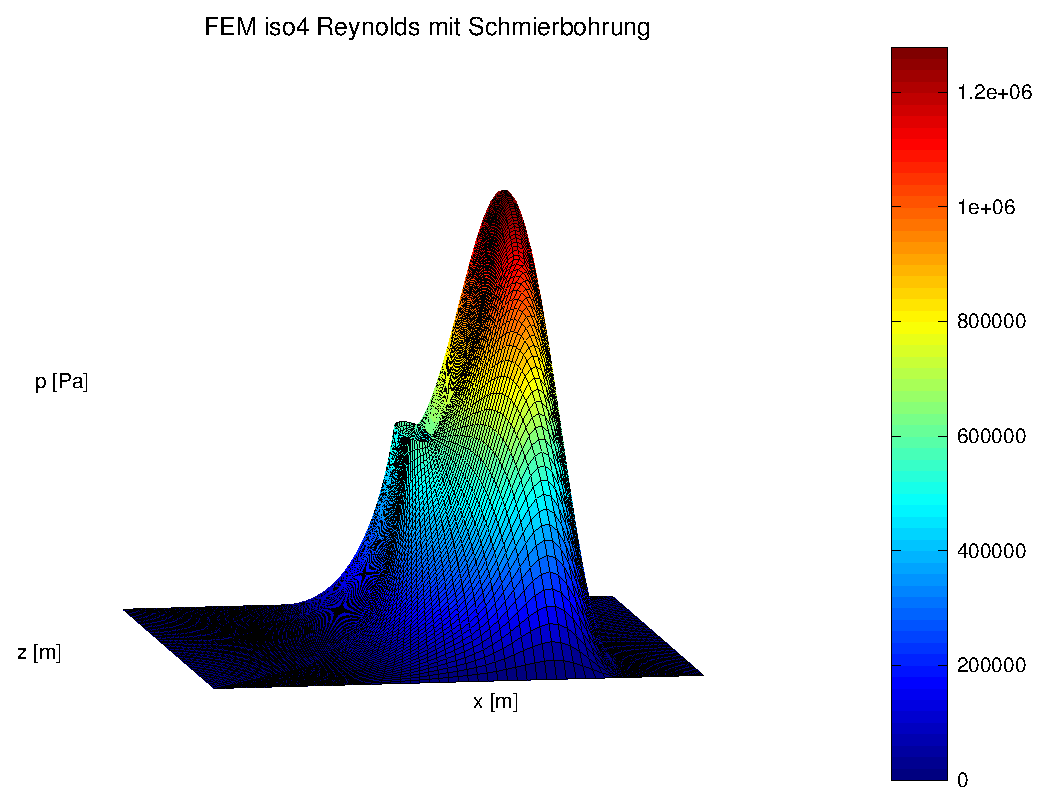
\includegraphics[width=\linewidth]{fig_hfe300}
\caption{Pressure distribution in the bearing with overpressure lubrication through a hole}
\label{fig:hfe_300}
\end{figure}

\section{Fluid structure interactions}
\label{sec:fsi_100}
In order to calculate the value of $w_{tot}$ which is needed for equation~\ref{eq:h_1400}, it is necessary to apply the pressure loads due to the hydrodynamic pressure $p$ and due to the contact pressure $p_{asp}$ to a Finite Element model for the bodies attached to the bearing shell and bearing journal respectively. The equations of motion of the Finite Element models must then be solved, and the resulting displacements can be used to calculate the total deformation $w_{tot}$ and its time derivative $\dot{w}_{tot}$. Since the hydraulic mesh used for the solution of the Reynolds equation can be attached either to the bearing journal or to the bearing shell, it is necessary to interpolate the total pressure $p_{tot} = p + p_{asp}$ from one body to the other. In the same way, it is necessary to interpolate the radial deformation $w_{2}$ in order to compute the total deformation $w_{tot}=w_1+w_2$.
\subsection{Reduced order models}
Because the bodies attached to the bearing shell and journal surface are assumed to undergo large rigid body motions, but the elastic deformations itself are assumed to be small and the material is assumed to be linear elastic, it is possible to apply model order reduction techniques in order to reduce the computational cost of the coupled fluid structure interaction problem. The software \href{https://github.com/octave-user/mboct-fem-pkg}{mboct-fem-pkg}, which is used to generate those reduced order models, implements a combined modal and static reduction based on \cite{Gash-1989}.
\subsubsection{Equations of motion with respect to the moving reference frame}
Despite the large rigid body motions of the bodies, the linear time invariant equations of motion~\ref{eq:fsi_100} of a representative body attached to the bearing shell or journal surface may be used as the basis of the model order reduction.
\begin{IEEEeqnarray}{rCl}
\label{eq:fsi_100}
\boldsymbol{M}_{fem} \, \ddot{\boldsymbol{U}}_{fem} + \boldsymbol{D}_{fem} \, \dot{\boldsymbol{U}}_{fem} + \boldsymbol{K}_{fem} \, \boldsymbol{U}_{fem} & = & \boldsymbol{R}_{fem}
\end{IEEEeqnarray}

\begin{IEEEeqnarray}{rCl}
\label{eq:fsi_200}
\boldsymbol{M}_{fem}&=&\begin{pmatrix}
\boldsymbol{M}_{11} & \boldsymbol{0} \\
\boldsymbol{0} & \boldsymbol{0}
\end{pmatrix} \\
\boldsymbol{D}_{fem}&=&\begin{pmatrix}
\boldsymbol{D}_{11} & \boldsymbol{0} \\
\boldsymbol{0} & \boldsymbol{0}
\end{pmatrix} \\
\boldsymbol{K}_{fem}&=&\begin{pmatrix}
\boldsymbol{K}_{11} & \boldsymbol{C}^T \\
\boldsymbol{C} & \boldsymbol{0}
\end{pmatrix} \\
\boldsymbol{U}_{fem}&=&\begin{pmatrix}
\boldsymbol{U}_{1} \\
\boldsymbol{\lambda}
\end{pmatrix} \\
\boldsymbol{R}_{fem}&=&\begin{pmatrix}
\boldsymbol{R}_{1} \\
\boldsymbol{U}_{pre}
\end{pmatrix}
\end{IEEEeqnarray}
\begin{description}
\item[$\boldsymbol{M}_{fem}$] Global mass matrix
\item[$\boldsymbol{D}_{fem}$] Global damping matrix
\item[$\boldsymbol{K}_{fem}$] Global stiffness matrix
\item[$\boldsymbol{R}_{fem}$] Global load vector
\item[$\boldsymbol{U}_{fem}$] Global displacement vector
\item[$\boldsymbol{M}_{11}$] Portion of the mass matrix related to all flexible degrees of freedom
\item[$\boldsymbol{D}_{11}$] Portion of the damping matrix related to all flexible degrees of freedom
\item[$\boldsymbol{K}_{11}$] Portion of the stiffness matrix related to all flexible degrees of freedom
\item[$\boldsymbol{C}$] Matrix of constraint equations
\item[$\boldsymbol{U}_1$] Portion of the displacement vector containing all flexible degrees of freedom
\item[$\boldsymbol{\lambda}$] Lagrange multipliers related to the constraint equations
\item[$\boldsymbol{R}_1$] Portion of the right hand side vector applied to all flexible degrees of freedom
\item[$\boldsymbol{U}_{pre}$] Portion of the right hand side vector related to imposed displacements and imposed rotations
\end{description}
\subsubsection{Constraint equations}
In order to perform a model order reduction, it is necessary to impose prescribed displacements at the surface of the bearing journal or bearing shell. This is achieved by means of load distributing coupling elements based on \cite{CODEASTERR30308}. All the constraint equations are assembled to the global $\boldsymbol{C}$ matrix.
\subsubsection{Static mode shapes}
The static mode shapes, needed for the model order reduction, are obtained by solving the linear system of equations~\ref{eq:fsi_300}. In equation~\ref{eq:fsi_300}, the identity matrix $\boldsymbol{I}_{pre}$ imposes unit displacements and rotations at the center of each bearing surface. However, it must be ensured that the resulting mode shapes $\boldsymbol{\varphi}_s$ do not contain any rigid body motions of the flexible body. Otherwise the modal stiffness matrix would become singular.
\begin{IEEEeqnarray}{rCl}
\label{eq:fsi_300}
\boldsymbol{\varphi}_s&=&\boldsymbol{K}_{fem}^{-1}\,\begin{pmatrix}\boldsymbol{0} \\
                                                                 \boldsymbol{I}_{pre}
                                                                 \end{pmatrix}
\end{IEEEeqnarray}
\subsubsection{Normal mode shapes}
In addition to the static mode shapes $\boldsymbol{\varphi}_s$, the dynamic mode shapes $\boldsymbol{\varphi}_n$ of the constrained flexible body are computed from the undamped general symmetric eigenvalue problem equation~\ref{eq:fsi_400}.
\begin{IEEEeqnarray}{rCl}
\label{eq:fsi_400}
\left(\boldsymbol{K}_{fem} - \lambda^2\,\boldsymbol{M}_{fem}\right)\,\boldsymbol{\varphi}_n & = & \boldsymbol{0}
\end{IEEEeqnarray}
\subsubsection{Pressure related mode shapes}
It is important to include additional mode shapes, in order to get a better representation of the deformations within the bearing surface. For that purpose the general symmetric eigenvalue problem~\ref{eq:fsi_500} is solved. See also \cite{Boedo-1997}.
\begin{IEEEeqnarray}{rCl}
\label{eq:fsi_500}
\left(\boldsymbol{K}_{fem} - \lambda\,\boldsymbol{A}_{diag}\right)\,\boldsymbol{\varphi}_p & = & \boldsymbol{0}
\end{IEEEeqnarray}
In order to get the diagonal matrix $\boldsymbol{A}_{diag}$, a load vector $\boldsymbol{R}_{p}$ is assembled with a uniform pressure load at the respective bearing surface. Then the components of the pressure load vector $\boldsymbol{R}_{p}$ are summed up and are stored at the diagonal of the matrix $\boldsymbol{A}$. All the nodes which are not within the respective bearing surface have zero entries at the diagonal of matrix $\boldsymbol{A}$. Typical mode shapes are shown in figure~\ref{fig:h1000} and figure~\ref{fig:h1100}.
\begin{IEEEeqnarray}{rCl}
\label{eq:fsi_600}
\boldsymbol{R}_{p}&=&\begin{pmatrix}
                        F_{x1} \\
                        F_{y1} \\
                        F_{z1} \\
                        \vdots{}
                     \end{pmatrix} \\
\boldsymbol{A}_{ii}&=&\sqrt{F_{xi}^2+F_{yi}^2+F_{zi}^2}
\end{IEEEeqnarray}

\begin{figure}[htb]
\centering
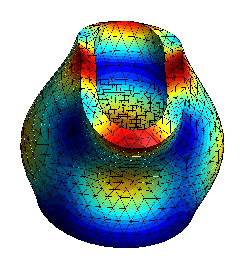
\includegraphics[width=0.25\linewidth]{fig_h1000}
\caption{Typical mode shape of a sleeve}
\label{fig:h1000}
\end{figure}

\begin{figure}[htb]
\centering
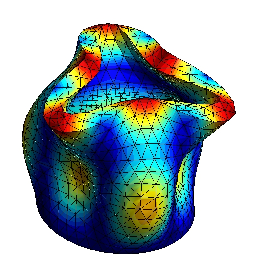
\includegraphics[width=0.25\linewidth]{fig_h1100}
\caption{Typical mode shape of a sleeve}
\label{fig:h1100}
\end{figure}

\subsubsection{Model order reduction}
Finally, all the different mode shapes $\boldsymbol{\varphi}_n$, $\boldsymbol{\varphi}_s$ and $\boldsymbol{\varphi}_p$ are combined in the model reduction matrix $\boldsymbol{T}_{red}$. It is important to note that the matrix $\boldsymbol{\varphi}_p$ is not necessarily orthogonal to $\boldsymbol{\varphi}_n$ and $\boldsymbol{\varphi}_s$. For that reason, it is necessary to apply a re-orthogonalization equation~\ref{eq:fsi_700}.
\begin{IEEEeqnarray}{rCl}
\boldsymbol{T}_{red}&=&\begin{pmatrix} \boldsymbol{\varphi}_n & \boldsymbol{\varphi}_s & \boldsymbol{\varphi}_p^{\star} \end{pmatrix} \\
\boldsymbol{\varphi}_p^{\star}&=&\boldsymbol{\varphi}_p - \boldsymbol{\varphi}_{ns} \, \left(\boldsymbol{\varphi}_{ns}^T\, \boldsymbol{M}_{fem}\,\boldsymbol{\varphi}_{ns}\right)^{-1}\,\boldsymbol{\varphi}_{ns}^T\, \boldsymbol{M}_{fem}\,\boldsymbol{\varphi}_{p} \label{eq:fsi_700} \\
\boldsymbol{\varphi}_{ns} & = & \begin{pmatrix} \boldsymbol{\varphi}_n & \boldsymbol{\varphi}_s \end{pmatrix}
\end{IEEEeqnarray}
Now, the reduced set of degrees of freedom $\boldsymbol{q}$ is defined and the model order reduction can be performed.
The reduced order matrices $\boldsymbol{M}_{red}$, $\boldsymbol{D}_{red}$ and $\boldsymbol{K}_{red}$ can be used directly for MBDyn's modal joint element described in section~\ref{sec:modal-element}.
\begin{IEEEeqnarray}{rCl}
\boldsymbol{U}_{fem}&\approx&\boldsymbol{T}_{red}\,\boldsymbol{q} \\
\underbrace{\boldsymbol{T}_{red}^T\,\boldsymbol{M}_{fem}\,\boldsymbol{T}_{red}}_{\boldsymbol{M}_{red}}\,\boldsymbol{\ddot{q}}+\underbrace{\boldsymbol{T}_{red}^T\,\boldsymbol{D}_{fem}\,\boldsymbol{T}_{red}}_{\boldsymbol{D}_{red}}\,\boldsymbol{\dot{q}}+\underbrace{\boldsymbol{T}_{red}^T\,\boldsymbol{K}\,\boldsymbol{T}_{red}}_{\boldsymbol{K}_{red}}\,\boldsymbol{q} & = & \underbrace{\boldsymbol{T}_{red}^T \, \boldsymbol{R}_{fem}}_{\boldsymbol{R}_{red}}
\end{IEEEeqnarray}
\subsection{Fluid structure interaction coupling matrices}
As described in section~\ref{sec:fsi_100}, it is necessary on one hand to apply the pressure loads at the bearing surface to the flexible body, and on the other hand to get the radial deformation from the flexible body in order to solve the Reynolds equation. This is achieved by means of the coupling matrices $\boldsymbol{D}$ and $\boldsymbol{E}$.
\begin{IEEEeqnarray}{rCl}
\boldsymbol{w}_i & = & \boldsymbol{D}_i \, \boldsymbol{q} \\
\boldsymbol{R}_{red} & = & \boldsymbol{R}_{red}^{\star} + \sum_{i=1}^{n}\boldsymbol{E}_i\,\boldsymbol{p}_{tot_i} \\
\boldsymbol{D}_{ij} & = & \boldsymbol{n}_{ij}^T \, \boldsymbol{T}_{red_{ij}} \\
\boldsymbol{E}_{i} & = & \boldsymbol{D}_{i}^T \, \boldsymbol{A}_i
\end{IEEEeqnarray}
\begin{description}
\item[$\boldsymbol{w}_i$] Vector of radial displacements at the surface of bearing~$i$
\item[$\boldsymbol{p}_{tot_i}$] Vector of the total pressure acting at the surface of bearing-$i$
\item[$\boldsymbol{D}_{i}$] Displacement coupling matrix for the surface of bearing~$i$
\item[$\boldsymbol{E}_{i}$] Pressure load coupling matrix for the surface of bearing~$i$
\item[$\boldsymbol{R}_{red}^{\star}$] Modal loads contributed by other elements including the modal joint itself.
\item[$\boldsymbol{n}_{ij}$] Surface normal vector at bearing surface~$i$ and node~$j$
\item[$\boldsymbol{A}_{i}$] Diagonal matrix of equivalent surface areas at bearing surface~$i$
\end{description}
\subsubsection{The global system of equations}
Equation~\ref{eq:fsi_750} to equation~\ref{eq:fsi_760} are showing an example for the global system of equations of motion of two flexible bodies connected with a hydrodynamic plain bearing.
All the terms marked with ``$a$'' are contributions from the hydrodynamic bearing element whereas the terms marked with ``$c$'' are contributions from the modal joint element.
The additional terms ``$b$'' are contributions from the automatic modal element. It is important to note that the pressure loads $\boldsymbol{E}_1 \, \boldsymbol{p}_{tot}$ and $\boldsymbol{E}_2 \, \boldsymbol{f}\left(\boldsymbol{p}_{tot}\right)$ do not contribute to the rigid body motion of the flexible bodies, but they contribute only to the deformations of the flexible bodies with respect to the moving reference frame. This moving reference frame is represented by a so called ``modal node'' and the equations of motion for the moving reference frame are equation~\ref{eq:fsi_755} - \ref{eq:fsi_760}. Since the reaction forces according to equation~\ref{eq:h310} - \ref{eq:h311}, \ref{eq:h410} - \ref{eq:h411}, \ref{eq:h420} - \ref{eq:h421} and \ref{eq:h430} - \ref{eq:h431} must contribute to the rigid body motion of the flexible bodies, these loads must be applied to the respective ``modal nodes'' attached to the modal joint elements.
\begin{IEEEeqnarray}{rCl}
\underbrace{-\boldsymbol{M}_{red_1} \, \ddot{\boldsymbol{q}}_1 - \boldsymbol{D}_{red_1} \, \dot{\boldsymbol{q}}_1 - \boldsymbol{K}_{red_1} \, \boldsymbol{q}_1 + \boldsymbol{R}_{red_1}^{\star}}_{c} + \underbrace{\boldsymbol{E}_1 \, \boldsymbol{p}_{tot}}_{a} &=&\boldsymbol{0}\label{eq:fsi_750}\\
\underbrace{-\boldsymbol{M}_{red_2} \, \ddot{\boldsymbol{q}}_2 - \boldsymbol{D}_{red_2} \, \dot{\boldsymbol{q}}_2 - \boldsymbol{K}_{red_2} \, \boldsymbol{q}_2 + \boldsymbol{R}_{red_2}^{\star}}_{c} + \underbrace{\boldsymbol{E}_2 \, f\left(\boldsymbol{p}_{tot}\right)}_{a} &=&\boldsymbol{0} \\
\underbrace{\boldsymbol{w}_{tot} - \boldsymbol{D}_1 \, \boldsymbol{q}_1 - \boldsymbol{f}\left(\boldsymbol{w}_2\right)}_{a} & = & \boldsymbol{0} \\
\underbrace{\boldsymbol{w}_2 - \boldsymbol{D}_2 \, \boldsymbol{q}_2}_{a} & = & \boldsymbol{0} \\
\underbrace{\boldsymbol{v}_1 - \dot{\boldsymbol{x}}_1}_{b} & = & \boldsymbol{0} \label{eq:fsi_755}\\
\underbrace{\boldsymbol{\omega}_1 - \boldsymbol{G}_1 \, \dot{\boldsymbol{g}}_1 - \Delta\boldsymbol{R}_1\,\boldsymbol{\omega}_{1_0}}_{b} & = & \boldsymbol{0} \\
\underbrace{-\dot{\boldsymbol{v}}_1\,m_1+\boldsymbol{S}_1 \times  \dot{\boldsymbol{\omega}}_1 - \boldsymbol{\omega}_1 \, \times \boldsymbol{\omega}_1 \times \boldsymbol{S}_1 + \boldsymbol{F}_{1}^{\star}}_{c} + \underbrace{\boldsymbol{F}_1}_{a} & = & \boldsymbol{0} \\
\underbrace{-\boldsymbol{J}_1 \, \dot{\boldsymbol{\omega}}_1 - \boldsymbol{S}_1 \times \dot{\boldsymbol{v}}_1 - \boldsymbol{\omega}_1 \times \boldsymbol{J}_1 \, \boldsymbol{\omega}_1 + \boldsymbol{M}_{1}^{\star}}_{c} + \underbrace{\boldsymbol{M}_1}_{a} & = & \boldsymbol{0} \\
\underbrace{\boldsymbol{v}_2 - \dot{\boldsymbol{x}}_2}_{b} & = & \boldsymbol{0} \\
\underbrace{\boldsymbol{\omega}_2 - \boldsymbol{G}_2 \, \dot{\boldsymbol{g}}_2 - \Delta\boldsymbol{R}_2\,\boldsymbol{\omega}_{2_0}}_{b} & = & \boldsymbol{0} \\
\underbrace{-\dot{\boldsymbol{v}}_2\,m_2+\boldsymbol{S}_2 \times  \dot{\boldsymbol{\omega}}_2 - \boldsymbol{\omega}_2 \, \times \boldsymbol{\omega}_2 \times \boldsymbol{S}_2 + \boldsymbol{F}_{2}^{\star}}_{c} + \underbrace{\boldsymbol{F}_2}_{a} & = & \boldsymbol{0} \\
\underbrace{-\boldsymbol{J}_2 \, \dot{\boldsymbol{\omega}}_2 - \boldsymbol{S}_2 \times \dot{\boldsymbol{v}}_2 - \boldsymbol{\omega}_2 \times \boldsymbol{J}_2 \, \boldsymbol{\omega}_2 + \boldsymbol{M}_{2}^{\star}}_{c} + \underbrace{\boldsymbol{M}_2}_{a} & = & \boldsymbol{0}\label{eq:fsi_760}
\end{IEEEeqnarray}
\begin{description}
\item[$\boldsymbol{R}_{red}^{\star}$] Additional contributions from the modal joint. See section~\ref{sec:modal-element}.
\item[$\boldsymbol{x}$] Position vector of a modal node
\item[$\boldsymbol{v}$] Velocity vector of a modal node
\item[$\Delta\boldsymbol{R}$] Rotation increment of a modal node. See section~\ref{sec:NodalRotation}.
\item[$\boldsymbol{\omega}$] Angular velocity vector of a modal node
\item[$\boldsymbol{G}$] A tensor related to rotation handling of the modal node. See section~\ref{sec:NodalRotation}.
\item[$m$] Total mass of the flexible body
\item[$\boldsymbol{S}$] Static moment of the flexible body
\item[$\boldsymbol{J}$] Inertia tensor of the flexible body
\item[$\boldsymbol{F}^{\star}$] Additional force contributions from the modal joint element. See section~\ref{sec:modal-element}
\item[$\boldsymbol{M}^{\star}$] Additional moment contributions form the modal joint element. See section~\ref{sec:modal-element}.
\end{description}
\subsubsection{Implementation}
It must be emphasized that the process of generating the matrices $\boldsymbol{M}_{red}$, $\boldsymbol{D}_{red}$, $\boldsymbol{K}_{red}$, $\boldsymbol{T}_{red}$, $\boldsymbol{D}$ and $\boldsymbol{E}$ is not built into MBDyn. For that purpose it is necessary to use the toolkit \href{https://github.com/octave-user/mboct-fem-pkg}{mboct-fem-pkg}.
The related function call to generate those matrices is ``fem\_ehd\_pre\_comp\_mat\_linear\_mesh''. Furthermore, the functions ``fem\_ehd\_pre\_comp\_mat\_export'' and ``fem\_cms\_export'' can be used to export all those matrices to a file format which can be read by MBDyn. See also MBDyn's \emph{input-manual}.

\subsection{Interpolation from the bearing journal to the bearing shell and vice versa}
It was mentioned in section~\ref{sec:fsi_100}, that the hydraulic mesh must be attached either to the bearing journal or to the bearing shell. Therefore, there remains the question of how to interpolate the total pressure $p_{tot}$ and the radial deformation $w_1$ from the bearing journal to the bearing shell for instance.
Actually MBDyn uses the interpolation according to R.J. Renka\cite{Renka-1988}.
\subsubsection{Construction of polynomials}
For each node at the hydraulic mesh, a polynomial function $C_{kl}$ is defined.
\begin{IEEEeqnarray}{rCl}
C_{kl}&=&f\left(x_{m_{kl}}, z_{m_{kl}}\right)+a_1\,\Delta x_{kl}^3 + a_2\,\Delta x_{kl}^2\,\Delta z_{kl}+a_3\,\Delta x_{kl}\,\Delta z_{kl}^2 \nonumber\\
&&+a_4\,\Delta z_{kl}^3+a_5\,\Delta x_{kl}^2+a_6\,\Delta x_{kl}\,\Delta z_{kl}+a_7\,\Delta z_{kl}^2+a_8\,\Delta x_{kl}+a_9\,\Delta z_{kl} \label{eq:fsi_800} \\
\boldsymbol{a}&=&\begin{pmatrix} a_1 & a_2 & a_3 & a_4 & a_5 & a_6 & a_7 & a_8\end{pmatrix}^T
\end{IEEEeqnarray}
\begin{description}
\item[$C_{kl}$] Polynomial function at the hydraulic node~$kl$ of the source mesh
\item[$f\left(x_{m_{kl}}, z_{m_{kl}}\right)$] Function (e.g. total pressure $p_{tot}$ or radial deformation at the moving mesh $w_{1}$) to be interpolated.
\item[$\boldsymbol{a}$] Coefficients of the polynomial
\end{description}
The coefficients $\boldsymbol{a}$ of the polynomial are fitted to the data to be interpolated.
\begin{IEEEeqnarray}{rCl}
\boldsymbol{a}&=&\boldsymbol{A}^{+}\,\Delta\boldsymbol{f} \\
\Delta f_{klm} & = & f_{klm} - f\left(x_{m_{kl}}, z_{m_{kl}}\right) \\
A_{mn}&=&\Delta x_{m}^{p_{x_n}}\,\Delta z_{m}^{p_{z_n}}
\end{IEEEeqnarray}
\begin{description}
\item[$\boldsymbol{A}$] A constant 16x9 matrix which is a function of the distances $\Delta x_{m}$ and $\Delta z_{m}$ between the central node, where the polynomial is constructed, and its neighbor nodes
\item[$\boldsymbol{A}^{+}$] The Moore-Penrose pseudo-inverse matrix of $\boldsymbol{A}$
\item[$p_x$] Exponents of the polynomial in $x$ direction
\item[$p_z$] Exponents of the polynomial in $z$ direction
\end{description}
\subsubsection{Interpolation}
According to \cite{Renka-1988}, the interpolated function $f$ is computed as a weighted average from several polynomials.
\begin{IEEEeqnarray}{rCl}
%% module-hydrodynamic_plain_bearing2.cc:13681
%% k -> kx
%% l -> kz
f\left(x_{f_i}, z_{f_j}\right)&=&\frac{fs_{ij}}{ws_{ij}} \\
fs_{ij}&=&\sum_{k=1}^{M}\sum_{l=1}^{N} \left(w_{kl}\right)^3\,C_{kl} \\
ws_{ij}&=&\sum_{k=1}^{M}\sum_{l=1}^{N} \left(w_{kl}\right)^3 \\
w_{kl}&=&\frac{R - d_{kl}}{R\,d_{kl}} \\
d_{kl}&=&\sqrt{\Delta x_{kl}^2 + \Delta z_{kl}^2} \\
\Delta x_{kl}&=&x_{f_i} - x_{m_{kl}} \\
\Delta z_{kl}&=&z_{f_j} - z_{m_{kl}}
%% x_{f_i}&=&x_i + \beta\, \Delta x_{m_1} \\
%% z_{f_j}&=&z_j + \beta\, \Delta x_{m_2} \\
\end{IEEEeqnarray}
\begin{description}
\item[$f$] Interpolated function
\item[$fs$] Weighted sum of the polynomial function
\item[$ws_{ij}$] Weighting factor
\item[$d_{kl}$] Total distance between the location of interpolation and the location where the polynomial is constructed
\item[$\Delta x_{kl}$] Distance in x-direction
\item[$\Delta z_{kl}$] Distance in z-direction
\end{description}
\subsubsection{Extrapolation}
In case of a piston to cylinder~liner contact, the axial movement of the piston is large compared to the size of the mesh, and it is necessary to evaluate the pressure outside the physical surface of the piston in order to apply a pressure load at the surface of the cylinder liner. For such a situation, the respective pressure boundary conditions at the boundaries of the bearing surface are used for the surface of the cylinder liner outside the physical surface of the piston. Since it is important to have a smooth transition of the boundary conditions, a transition region with an axial extent of $2\,\epsilon$ is defined. Within the transition region, an interpolation between the boundary condition and the data from the mesh is performed.
\begin{IEEEeqnarray}{rCl}
f^{\star}\left(x_{f_i}, z_{f_j}\right)&=&\alpha\,f\left(x_{f_i}, z_{f_j}\right) + \left(1 - \alpha\right) \, f_{bc} \\
\end{IEEEeqnarray}
\begin{description}
\item[$f^{\star}$] Modified interpolation function
\item[$\alpha$] Interpolation coefficient
\item[$\epsilon$] Transition area
\item[$f_{bc}$] Function value provided by the boundary condition
\end{description}
The interpolation coefficient is defined as:
\begin{IEEEeqnarray}{rCl}
\alpha&=&\left\vert \begin{array}{ccccc}
1 & \text{if} & -\frac{1}{2} \, B + \epsilon \le z_{f_i} \le \frac{B}{2} - \epsilon \\
0 & \text{if} & z_{f_i} > \frac{B}{2} + \epsilon & \text{or} & z_{f_i} < -\frac{B}{2} - \epsilon \\
\frac{z_{f_j} + \frac{B}{2} + \epsilon}{2 \, \epsilon} & \text{if} & -\frac{B}{2} - \epsilon \le z_{f_i} \le -\frac{B}{2} + \epsilon \\
\frac{\frac{B}{2} + \epsilon - z_{f_i}}{2 \, \epsilon} & \text{if} & \frac{B}{2} - \epsilon \le z_{f_i} \le \frac{B}{2} + \epsilon
\end{array}\right.
\end{IEEEeqnarray}
